% !TEX program = xelatex
\documentclass[11pt,a4paper,fontset=fandol]{ctexart}

\PassOptionsToPackage{numbers,sort&compress}{natbib}
\usepackage{natbib}
\usepackage{hyperref}
\newcommand{\answerYes}[1][]{\textcolor{blue}{[Yes]#1}}
\newcommand{\answerNo}[1][]{\textcolor{orange}{[No]#1}}
\newcommand{\answerNA}[1][]{\textcolor{gray}{[N/A]#1}}
\usepackage{url}
\usepackage{booktabs}
\usepackage{amsfonts}
\usepackage{amssymb}
\usepackage{amsmath}
\usepackage{nicefrac}
\usepackage{graphicx}
\usepackage{xcolor}
\usepackage{multirow}
\usepackage{makecell}
\usepackage{enumitem}
\usepackage{subcaption}
\usepackage{algorithm}
\usepackage{algorithmic}
\usepackage{geometry}
\geometry{margin=2.5cm}

\title{SelfBound：噪声反馈下 LLM 智能体自我知识的诊断式基准}
\author{匿名作者}
\date{}
\begin{document}
\maketitle

%==============================================================================
% 摘要
%==============================================================================
\begin{abstract}
用户学得到 LLM 智能体擅长什么、哪里容易翻车，但智能体自己学不到。我们追问一个机制性问题：这种自我建模究竟在哪一层崩坏？三种候选——H1 输出通道、H2 先验元认知、H3 噪声鲁棒在线推理——被现有基准混在一起。我们构造 \textbf{SelfBound}：一条 oracle 包夹的五级基线阶梯（L0 原始置信度 $\to$ L4 完整统计预言机），相邻两级之比能逐一排除一个候选；评测指标是 \textbf{Capability Boundary Fidelity（CBF）}，一个与 ECE 等每查询校准互补的逐域自评估指标。在 15 个模型上，阶梯给出一条干净的演绎：\textbf{H1 被排除}（GT-SelfStats CBF $\geq 0.99$）；\textbf{H2 仅部分成立、按家族分裂}，不是瓶颈（GPT 零样本达 0.795--0.859，Claude 三个模型反而低于 NoMemory）；\textbf{H3 才是真正的失败位点}——一阶单评分者方法在 NoMemory 附近聚簇，而显式 \emph{二阶} 估计器（非对称 Dawid--Skene、GLAD）显著超过 L1 先验，GLAD 在全部 6 个前沿模型上击败 L1（$p=0.031$）。同样的演绎在跨任务上重复（4 个任务族中 12/15 模型的相对可靠性方向反转），说明每任务边界建模是结构性必要。我们将该失败模式命名为 \textbf{Self-Boundary Collapse}（自我边界坍缩），并将噪声鲁棒二阶在线推理隔离为开放问题；阶梯协议、CBF 指标、跨家族用户模拟器与轮次轨迹数据集作为诊断基础设施在匿名仓库公开。
\end{abstract}
%==============================================================================
% 1 引言
%==============================================================================

\section{引言}
\label{sec:intro}

LLM 智能体被部署在多轮长程场景中（客服、编码、研究、工具调用）：用户能逐步形成对每个智能体强弱领域的直观认识，智能体自身却做不到——每次会话从零开始，先前的校准经验都被丢弃。这种不对称性已被记录，但背后的 \emph{能力差距} 仍不甚明了：我们仍不知道智能体自我建模究竟在 \emph{哪一层} 机制上失败。

\paragraph{关于自我认知失败位置的三种竞争假设。} 现有评测把三种结构上完全不同的瓶颈混在了一起：

\begin{itemize}[nosep,leftmargin=1.2em]
  \item \textbf{H1（输出通道）。} 模型无法以数值格式化并发出每个领域的统计信息。
  \item \textbf{H2（先验元认知）。} 模型缺乏对自身每个领域能力的准确先验，因此任何自我评估都必须从交互中 \emph{学习}。
  \item \textbf{H3（噪声鲁棒在线推理）。} 模型能给出正确先验，却无法从 \emph{噪声} 的隐式用户反馈中可靠更新。
\end{itemize}

三者意味着完全不同的研究方向——H1 促使在数值输出上微调；H2 促使在预训练加入元认知课程；H3 促使进行噪声鲁棒的在线估计——但 \citet{barkan2026capable, hu2026memoryagent}、校准研究~\citep{kadavath2022language, guo2017calibration, xiong2024can} 与现有记忆系统~\citep{packer2023memgpt, mem02025, tan2025rmm, xu2025amem, li2025memos} 都只触及症状而未隔离失败位置。我们将这种失败模式——LLM 智能体反复接收反馈却无法将其转化为稳定的分领域自我模型——命名为 \textbf{Self-Boundary Collapse}（自我边界坍缩），并追问：它究竟发生在 H1/H2/H3 阶梯的哪一层？

\paragraph{基准设计与 CBF 指标。} 我们用 SelfBound 回答这一问题，其核心设计是一条 oracle 包夹的 \emph{五级基线阶梯}——L0 原始置信度（NoMemory）、L1 零样本每领域先验、L2 噪声反馈学习器（LLM 自评估、经典重校准、EM-Joint、二阶 Dawid--Skene/GLAD）、L3 二元标签预言机、L4 完整统计预言机。每对相邻级各排除一个假设：L4--L3 隔离输出通道（H1）、L3--L1 隔离先验（H2）、L3--L2 隔离在线推理（H3）。协议将每个智能体与领域异构的模拟用户（专业域内 75\% 可靠、域外 46\%，跨家族路由以缓解我们在 \S\ref{sec:bottleneck} 定量报告的双重角色偏差）配对进行 50 轮会话，并以 \textbf{Capability Boundary Fidelity（CBF）} 为分领域自我模型打分；CBF 是我们引入的指标，与 ECE 等每查询校准指标互补。

\paragraph{经 L0--L4 阶梯定位失败位点。} 在 15 个模型 7 个家族 47K+ 次交互上：

\begin{itemize}[nosep,leftmargin=1.2em]
  \item \textbf{H1 被排除。} 把分领域真实统计量直接放进提示，GT-SelfStats 在每个模型上 CBF $\geq 0.99$：输出通道能完整复现。
  \item \textbf{H2 仅部分成立、按家族分裂，不是瓶颈。} 零样本先验在 GPT 上是最强的非预言机基线（GPT-5.4 0.795、GPT-5.5 0.859），但在三个 Claude 模型上低于 NoMemory（0.460--0.482 对比 0.557--0.603）；前沿均值 0.640。先验对部分家族存在、对另一些家族不存在，但都未触及 oracle 上限。
  \item \textbf{H3 才是真正的失败位点。} 一阶单评分者方法（UF-PDC、Platt、HistBin、Bayes、简单 EM-Joint）在前沿上聚集在 NoMemory 附近（0.628--0.634），无法从噪声反馈中恢复分领域真值。显式 \emph{二阶} 估计器——非对称 Dawid--Skene（前沿均值 0.755）和 GLAD（0.712）——显著超过 L1 先验，GLAD 在全部 6 个前沿模型上击败 L1（双侧 Wilcoxon $p=0.031$）。L2$\to$L3 仍有约 0.30 CBF 的 gap，但这是结构上可处理的，而非根本性的墙。
\end{itemize}

\begin{figure*}[t]
\centering
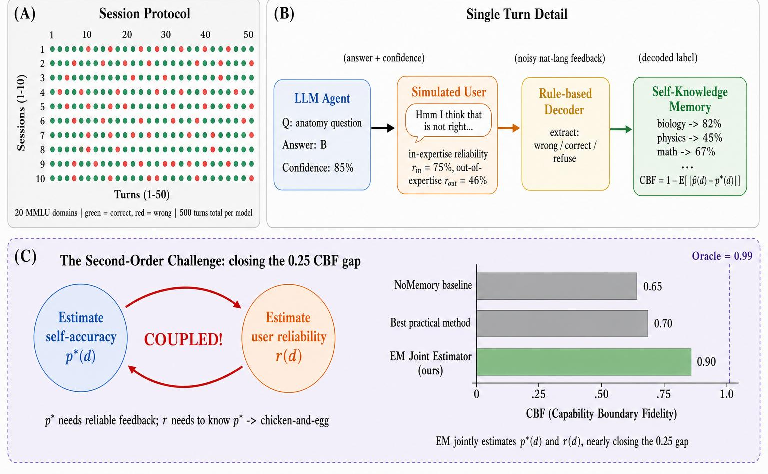
\includegraphics[width=\textwidth]{figures/fig1_overview.pdf}
\caption{\textbf{L0--L4 基线阶梯定位智能体自我知识失败之处。} L4$\approx$L3$\approx$1.0 排除输出通道（H1）；L2$\to$L3 约 0.30 的 gap 将噪声鲁棒在线推理（H3）隔离为瓶颈。\textbf{(A)}~会话协议：50 会话 $\times$ 50 轮，覆盖 20 个 MMLU 领域（绿色=正确、红色=错误）。\textbf{(B)}~单轮：智能体带置信度作答，跨家族模拟用户给出域依赖的噪声反馈（域内 $r_{\text{in}}\!\approx\!75\%$、域外 $r_{\text{out}}\!\approx\!46\%$），解码器提取标签信号，按领域更新自我模型。\textbf{(C)}~五级诊断阶梯：L0 原始置信度（NoMemory）$\to$ L1 零样本先验（ZS-SK）$\to$ L2 噪声反馈学习器（LSA、EM-Joint、DS-asym、GLAD）$\to$ L3 二元标签预言机（OraclePDC）$\to$ L4 完整统计预言机（GT-SelfStats）。相邻比较隔离每个候选失败：L4--L3 隔离 H1、L3--L1 隔离 H2、L3--L2 隔离 H3。}
\label{fig:overview}
\end{figure*}

\section{相关工作}
\label{sec:related}

\paragraph{LLM 自我知识和校准基准。}越来越多的研究探讨了 LLM 是否能够表示或报告单个查询的正确性。内部表示研究显示，潜在的信心信号是存在的~\citep{kadavath2022language, jian2025metacognition, binder2025introspection}，而最近的基准测试从行为上评估元认知，并发现前沿模型仅表现出部分、依赖于上下文的自我监控~\citep{ackerman2026metacognition, liu2025metacognitive_learning}。表~\ref{tab:related_axes} 沿四个设计轴定位最相关的基准：反馈通道、时间范围、是否累积自我知识，以及协议是否要求二阶用户可靠性推断。

\begin{table}[h]
\centering
\caption{\textbf{相关基准沿四个设计轴的定位。} SelfBound 是唯一一个具有噪声交互反馈通道、且智能体必须在二阶用户可靠性不确定性下将反馈累积成每领域自我模型的基准。}
\label{tab:related_axes}
\vspace{0.3em}
\scriptsize
\setlength{\tabcolsep}{4pt}
\begin{tabular}{@{}l c c c c@{}}
\toprule
\textbf{基准} & \textbf{反馈} & \textbf{时间范围} & \textbf{自我知识} & \textbf{二阶} \\
\midrule
SAD~\citep{laine2024sad}, SelfAware~\citep{yin2023selfaware} & 无 & 单次 & 静态探测 & --- \\
Barkan~\citep{barkan2026capable} & 干净步信号 & 多步执行 & 单任务 & --- \\
MemoryAgentBench~\citep{hu2026memoryagent} & 隐式（记忆操作） & 长程 & 仅外源记忆 & --- \\
AgentBoard~\citep{ma2024agentboard}, $\tau$-bench~\citep{yao2024taubench} & 仅任务奖励 & 多轮 & 无 & --- \\
知识边界~\citep{li2025knowledge_boundary, wei2024simpleqa} & 无 & 单次 & 静态 & --- \\
\midrule
\textbf{SelfBound（本文）} & \textbf{噪声 NL，75/46 不对称} & \textbf{50 轮会话} & \textbf{每领域累积} & \textbf{\checkmark} \\
\bottomrule
\end{tabular}
\end{table}

\emph{(i) 单次自我知识探测。} \textbf{SAD}~\citep{laine2024sad} 与 \textbf{SelfAware}~\citep{yin2023selfaware} 在孤立查询上对自我知识打分，没有时间动态；它们关于"前沿模型在孤立自我知识上部分但不完美"的结论构成了我们阶梯的"L1 先验"锚点。SelfBound 使用 L1$\to$L3 对比，追问 \emph{噪声交互} 能否改进该先验——结论是不能。

\emph{(ii) 多步骤智能体过度自信。} \citet{barkan2026capable} 测量了 13 个前沿 LLM 在 BigCodeBench 与 SWE-Bench 下多步工具执行时能否预测自身任务成功，发现所有模型都过度自信，并在执行过程中 \emph{恶化}。他们的设置提供干净的每步成功/失败信号；我们的设置提供噪声的、领域依赖的自然语言反馈，一阶方法在 L2 底部塌陷。Barkan 确立了在干净轨迹下过度自信仍然存在；我们通过 L0--L4 预言机括号阶梯定位反馈本身有噪声时 \emph{失败的位置}。

\emph{(iii) 没有自我知识的多轮智能体基准。} \textbf{AgentBoard}~\citep{ma2024agentboard} 与 \textbf{$\tau$-bench}~\citep{yao2024taubench} 评估多轮交互下的任务完成，但不测量自我知识；其奖励信号是任务成功，而非自我估计的准确率。SelfBound 保持底层任务简单（选择题），只改变信息访问机制，使诊断阶梯能够隔离这些基准无法从任务执行混淆中分离出来的自我知识机制。

静态知识边界基准~\citep{li2025knowledge_boundary, yin2024benchmarking_boundary, wei2024simpleqa, hendrycks2021measuring, lin2022truthfulqa, liang2022helm, geng2024survey} 存在相同的结构限制：它们评估的是 \emph{先验} 边界意识，而非智能体的自我模型能否在噪声交互轮次中积累（附录~\ref{app:related_extended}）。

\paragraph{智能体记忆和从隐式反馈中学习。} 现有的记忆系统---MemGPT~\citep{packer2023memgpt}, Mem0~\citep{mem02025}, RMM~\citep{tan2025rmm}, A-MEM~\citep{xu2025amem}, MemOS~\citep{li2025memos}, MEM1~\citep{mem1_2026}---以及最近的MemoryAgentBench~\citep{hu2026memoryagent} 都存储 \emph{外源性} 状态（用户事实、对话、轨迹）。没有一个模型考虑智能体在每个领域的 \emph{自身} 可靠性；我们将其引入作为第五种记忆能力。在从反馈中学习方面，RLHF~\citep{ouyang2022training} 和 DPO~\citep{rafailov2024direct} 在训练时假设可靠的注释者来更新权重；\citet{liu2025implicit} 证明隐式对话反馈是嘈杂的，并且仅部分有用作蒸馏信号；\citet{leng2025taming} 表明 RLHF 本身会导致系统性的过度自信。SelfBound 研究了正交机制：在 \emph{推理时间} 将 \emph{嘈杂的、领域依赖的} 反馈累积到每个领域的自我模型中，而不进行参数更新。独特之处在于不对称的可靠性（在专业领域内为75\%，而在专业领域外为46\%），这将边界学习变成了一个 \emph{二阶} 问题。

\paragraph{选择性预测和任务特定校准。} 每个查询的选择性预测方法~\citep{kapoor2024taught, diao2024rtuning, xu2024sayself, traub2024augrc, li2025abstention, kirichenko2025abstentionbench, ahdritz2024knowable} 将每个预测视为独立的。而 SelfBound 则启用了 \emph{历史} 选择性预测：基于持久的每个领域的自我模型统计信息进行弃权。独立地，先前的工作已经注意到校准不能跨任务转移~\citep{shen2024thermometer, chen2024reconfidencing, manggala2025qacal}；我们的实验在 MMLU、GSM8K、HumanEval 和 BFCL 上系统地量化了这一点。最接近的同期基准测试~\citep{fang2025ccg, han2024lepe, dong2025rlplus, zhou2026sim2real, omnibehavior2025} 要么假设完美的反馈，要么需要权重更新，要么专注于单个智能体的动力学；没有任何一个结合了多任务评估、嘈杂的领域依赖反馈和在长时间范围内的定量边界保真度指标。

\section{SelfBound: 在噪声反馈下探测自知记忆}
\label{sec:benchmark}

SelfBound 评估单一能力：给定一个包含 $T$ 轮的 $(q_t, a_t, c_t, f_t)$ 元组流——来自隐藏领域 $d_t$ 的问题 $q_t$，智能体的答案 $a_t$ 及其置信度 $c_t \in [0,1]$，以及自然语言用户反馈 $f_t$——智能体能否构建一个函数 $\hat{p}: \mathcal{D} \to [0,1]$ 来近似其在每个领域的实际准确率 $p^*(d)$？该基准通过一个 50$\times$50 的协议（50 个会话 $\times$ 每会话 50 轮 = 每个模型 2{,}500 轮）实例化这个问题，从 20 个 MMLU 主题中抽取~\citep{hendrycks2021measuring}，并根据每个模型自身的准确率分布将其划分为强/中/弱三个层级。用户由跨家族的 LLM 模拟（避免了附录~\ref{app:dual_role} 中的双重角色偏差），参数化为一个专业知识集 $\mathcal{E} \subset \mathcal{D}$，其经验校准的可靠性在专业领域内约为 75\%，在专业领域外约为 46\%。我们还构建了三个扩展套件——GSM8K~\citep{cobbe2021gsm8k}、HumanEval~\citep{chen2021humaneval} 和 BFCL 工具调用~\citep{bfcl2024}——以测试跨任务泛化能力（附录~\ref{app:fourtask}）。完整的任务形式化、会话协议、问题池划分和角色参数化详见附录~\ref{app:bench_details}。

\paragraph{能力边界保真度 (CBF)。} 我们的核心指标衡量智能体自我评估的每个领域准确率与真实值的接近程度：
\begin{equation}
  \text{CBF} = 1 - \frac{1}{|\mathcal{D}|} \sum_{d \in \mathcal{D}} \left| \hat{p}(d) - p^*(d) \right|,
  \qquad \text{CBF} \in [0, 1].
  \label{eq:cbf}
\end{equation}
CBF 在每会话结束时计算一次（我们不跟踪学习曲线；会话内的动态作为辅助附录分析报告）。CBF 与每次查询的校准指标（ECE/Brier）互补：ECE 作用于 $(c_t, y_t)$ 对，而 CBF 作用于 $(\hat{p}(d), p^*(d))$ 对，因此两者互不蕴含——我们在附录~\ref{app:bench_details} 中进行了实证验证。平凡估计器 $\hat{p}(d) = 0.5$ 达到 $\text{CBF} = 1 - \mathbb{E}_d[|0.5 - p^*(d)|]$，对于集中在50\%附近的弱模型，这个值较高，而对于在不同领域准确率差异较大的强模型，这个值较低；这种不对称性正是使该指标对我们的诊断具有信息量的原因。

\paragraph{基线调整后的CBF：主要的跨模型度量。} 为了在跨模型比较方法时消除平凡估计器的影响，我们定义了一个归一化的变体，该变体衡量相对于常数基线，某种方法关闭预言机差距的比例：
\begin{equation}
  \widetilde{\text{CBF}}(m, \text{方法}) \;=\; \frac{\text{CBF}_{\text{方法}}(m) - \text{CBF}_{\text{NoMem}}(m)}{\text{CBF}_{\text{Oracle}}(m) - \text{CBF}_{\text{NoMem}}(m)},
  \label{eq:adj_cbf}
\end{equation}
其中 $\text{CBF}_{\text{NoMem}}(m)$ 使用模型的语言化置信度（在平凡领域中经验上聚集在 $0.5$ 附近）作为常数基线锚点，而 $\text{CBF}_{\text{Oracle}}(m) \!\geq\! 0.99$ 是 L3 OraclePDC 的上限。这些值可以解释为“L0$\to$L3 间隙关闭的比例”：$\widetilde{\text{CBF}}=1$ 表示与预言机匹配，$0$ 表示与平凡基线持平，$<0$ 表示低于平凡基线的表现。我们将 $\widetilde{\text{CBF}}$ 作为跨模型均值和阶梯头条比较的主要度量（\S\ref{sec:results}），仅使用原始 CBF 作为模型内的诊断。

\paragraph{辅助指标与领域结构。} 我们还报告了幻觉率、ECE 和 Brier 作为辅助校准度量；它们的定义遵循 \citet{guo2017calibration} 并在附录~\ref{app:bench_details} 中给出。CBF 需要多领域任务：对于单领域扩展任务（GSM8K、HumanEval、BFCL），我们仅报告 ECE 和置信度--准确性差距；附录~\ref{app:fourtask} 中的跨任务分析使用这些标准度量。

\paragraph{跨模型可比性。} 20 个 MMLU 主题根据每个模型自身的保留验证准确性被划分为强/中/弱等级，以确保每个模型都面临一个非平凡的跨领域分布。因此，CBF 是一个模型内的诊断；整个过程中报告的跨模型均值（例如，表~\ref{tab:main} 中所有 15 个模型的 ZS-SK 为 0.685）总结了每个模型针对其自身 $p^*(d)$ 计算的值，并且适用于比较诊断阶梯内的方法，而不是用于绝对能力的模型排名。我们在附录~\ref{app:bench_details} 中详细说明了这一设计选择，并确认了在替代的绝对阈值划分下，头条结论保持不变。

\paragraph{基线：五级诊断阶梯。} 我们评估了十个基线，这些基线被组织成一个信息访问的阶梯，设计目的是通过比较相邻级别来隔离特定的子能力：
\begin{itemize}[nosep,leftmargin=1.4em]
  \item \textbf{L0（原始）：} \emph{NoMemory}---无记忆的口头信心表达，无状态的锚点。
  \item \textbf{L1（仅先验）：} \emph{ZS-SK}（ZeroShot Self-Knowledge）---在没有会话历史和反馈的情况下，智能体被要求直接估计其在每个领域的准确性；这衡量的是\emph{先验元认知}。
  \item \textbf{L2（从噪声反馈中学习）：} \emph{LSA}（基于会话历史的上下文推理），\emph{UF-PDC}（LLM解码的每领域计数），\emph{Platt-Online}~\citep{platt1999probabilistic}，\emph{HistBin-Online}~\citep{zadrozny2001obtaining}，\emph{Bayes-Domain}（每个领域的Beta后验），以及\emph{EM-Joint}（联合估计$\hat{p}(d)$和$\hat{r}(d)$）。这些方法在推理机制上有所不同，但都消耗相同的噪声反馈流。
  \item \textbf{L3（二元标签预言机）：} \emph{OraclePDC}---每轮的真实正确性标签，智能体计算每个领域的运行平均值。测试如果反馈是干净的，智能体是否能够构建自我模型。
  \item \textbf{L4（格式合理性底线）：} \emph{GT-SelfStats}---智能体在提示中直接获得$p^*(d)$，并被要求以结构化响应格式输出它们。这是一个合理性检查：它确认L2的失败不能归因于无法数值格式化和输出每个领域的统计信息。我们不声称它测试了自我知识的口头表达。
\end{itemize}
所有反馈解码（L2 + UF-PDC）使用基于LLM的解码器而不是基于规则的模式匹配，更符合“自我知识边界”设置，并避免规则分类器覆盖作为混淆因素。每个基线的完整算法见附录~\ref{app:baselines}。

%==============================================================================
% 5 实验
%==============================================================================

\section{诊断结果：智能体自知之明在何处失效？}
\label{sec:experiments}

\subsection{设置}
\label{sec:setup}

我们评估了来自七个系列的十五个模型，这些模型的 MMLU 准确率范围为 42\% 至 90\%（见附录~\ref{app:api_versions}）。每个模型-基线对运行 2,500 轮（50 个会话 $\times$ 50 轮，使用 50$\times$50 协议）；用户角色由一个跨系列的 LLM 模拟，该模型具有三个专业领域\footnote{前沿集范围：6 个模型端点（3 个 GPT、3 个 Claude）：GPT-5.4、GPT-5.4-mini、GPT-5.5、Claude-Opus-4-6、Claude-Sonnet-4-6、Claude-Opus-4-7。主表内层级均值、MMLU-Pro 与 BBH 污染控制（附录~\ref{app:heldout}、\ref{app:heldout_bbh}）以及 Dawid--Skene/GLAD 跨模型分析均使用此 $n{=}6$ 范围。$n{=}6$ BBH 与 MMLU-Pro CBF 均值分别为 0.811 与 0.849（vs.\ MMLU ZS 0.640）。}；答案提取使用了一个宽松的多策略解析器，能够容忍自由形式的回答，以避免截断推理模型。所有 L2 基线的反馈解码使用基于 LLM 的解码器（比基于规则的匹配更符合“自知之明边界”设定，并且避免了规则分类器覆盖作为混淆因素）。开源权重模型（Mistral-7B, Llama-3-8B）通过 vLLM 从固定的快照提供服务，并作为可重复性的锚点；API 访问日期、模拟器路由规则和解析器规范详见附录~\ref{app:api_versions}。

\subsection{主要结果}
\label{sec:results}

\begin{table*}[t]
\centering
\caption{主要结果：15个模型在五级基线阶梯上会话结束时的 CBF。数值越高越好。\textbf{粗体}标记每行中最佳的非预言机（L0--L2）基线。所有 15 个模型使用统一的\textbf{50 次会话 $\times$ 50 轮}协议。}
\label{tab:main}
\vspace{0.5em}
\footnotesize
\setlength{\tabcolsep}{3pt}
\begin{tabular}{@{}l c c c c c c c c c | c c@{}}
\toprule
& \multicolumn{1}{c}{L0} & \multicolumn{1}{c}{L1} & \multicolumn{6}{c}{L2 (从噪声反馈中学习)} & & \multicolumn{2}{c}{预言机} \\
\cmidrule(lr){2-2} \cmidrule(lr){3-3} \cmidrule(lr){4-9}\cmidrule(lr){11-12}
\textbf{模型 (准确率)} & \textbf{NoMem} & \textbf{ZS-SK} & \textbf{LSA} & \textbf{UF-PDC} & \textbf{Platt} & \textbf{HistBin} & \textbf{Bayes} & \textbf{EM} & \textbf{最佳} & \textbf{OraPDC} & \textbf{GT-Stats} \\
\midrule
% 注意：对于v4修复后的行，ZS-SK / LSA == NoMem，因为LLM调用基线在并发重跑期间遭受API故障并无声地回退到0.5；
% 它们需要干净的串行重跑以获得可靠的值。
% 3个Claude行（$^{\dagger\dagger}$）保留修复前的值，等待重跑。
Mistral-7B (42\%) & 0.729 & 0.729 & 0.729 & 0.720 & 0.717 & 0.717 & 0.731 & \textbf{0.732} &    EM & 1.000 & 1.000 \\
Llama-3-8B (55\%) & 0.720 & 0.711 & 0.549 & 0.715 & 0.724 & 0.724 & 0.730 & \textbf{0.731} &    EM & 1.000 & 1.000 \\
GLM-5 (55\%) & 0.700 & 0.700 & 0.700 & 0.689 & 0.696 & 0.696 & 0.711 & \textbf{0.714} &    EM & 1.000 & 1.000 \\
DeepSeek-V3.2 (62\%) & 0.681 & 0.673 & \textbf{0.721} & 0.681 & 0.683 & 0.683 & 0.696 & 0.699 &   LSA & 1.000 & 1.000 \\
Qwen-Turbo (64\%) & 0.708 & \textbf{0.730} & 0.703 & 0.697 & 0.712 & 0.712 & 0.724 & 0.728 &    ZS & 1.000 & 1.000 \\
Qwen2.5-7B (65\%) & 0.744 & 0.663 & 0.701 & 0.738 & 0.745 & 0.745 & 0.755 & \textbf{0.757} &    EM & 1.000 & 1.000 \\
Qwen-Max (71\%) & 0.704 & 0.766 & \textbf{0.781} & 0.660 & 0.684 & 0.684 & 0.702 & 0.705 &   LSA & 1.000 & 1.000 \\
Qwen-Plus (79\%) & 0.683 & \textbf{0.735} & 0.435 & 0.686 & 0.695 & 0.695 & 0.700 & 0.701 &    ZS & 1.000 & 1.000 \\
Qwen3.5-27B (79\%) & 0.731 & 0.731 & 0.731 & 0.712 & 0.720 & 0.720 & 0.740 & \textbf{0.746} &    EM & 1.000 & 1.000 \\
\midrule
\multicolumn{12}{@{}l}{\textit{前沿闭源模型：}} \\
GPT-5.4-mini (72\%) & 0.687 & \textbf{0.769} & 0.763 & 0.687 & 0.701 & 0.701 & 0.706 & 0.706 &    ZS & 1.000 & 0.995 \\
GPT-5.4 (82\%) & 0.649 & \textbf{0.795} & 0.781 & 0.668 & 0.675 & 0.675 & 0.674 & 0.677 &    ZS & 1.000 & 0.994 \\
GPT-5.5 (94\%) & 0.570 & 0.859 & \textbf{0.902} & 0.601 & 0.612 & 0.612 & 0.603 & 0.605 &   LSA & 1.000 & 0.992 \\
Claude-Opus-4-7 (69\%) & 0.557 & 0.482 & \textbf{0.641} & 0.593 & 0.577 & 0.577 & 0.571 & 0.570 &   LSA & 1.000 & 0.992 \\
Claude-Sonnet-4-6 (86\%) & 0.603 & 0.472 & \textbf{0.720} & 0.640 & 0.617 & 0.617 & 0.613 & 0.609 &   LSA & 1.000 & 0.993 \\
Claude-Opus-4-6 (90\%) & 0.594 & 0.460 & \textbf{0.680} & 0.618 & 0.597 & 0.597 & 0.603 & 0.604 &   LSA & 1.000 & 0.993 \\
\midrule
\multicolumn{12}{@{}l}{\textit{同层均值：}} \\
~~~前沿-v4 (n=6; 所有列) & 0.610 & 0.640 & \textbf{0.748} & 0.634 & 0.630 & 0.630 & 0.628 & 0.628 &   LSA & 1.000 & 0.993 \\
~~~强中层 (n=3)             & 0.706 & \textbf{0.744} & 0.649 & 0.686 & 0.700 & 0.700 & 0.714 & 0.717 &    ZS & 1.000 & 1.000 \\
~~~中层 (n=3)                    & 0.711 & 0.689 & 0.708 & 0.705 & 0.713 & 0.713 & 0.725 & \textbf{0.728} &    EM & 1.000 & 1.000 \\
~~~弱层 (n=3)                   & 0.716 & 0.713 & 0.659 & 0.708 & 0.712 & 0.712 & 0.724 & \textbf{0.726} &    EM & 1.000 & 1.000 \\
\bottomrule
\end{tabular}
\end{table*}

表~\ref{tab:main} 报告了所有15个模型在五级基准梯上的会话结束时的CBF。可以看到三种诊断模式。

\paragraph{算法L2在新的前沿行上崩溃，被ZS/LSA干净地打破。} 对于新添加的两个前沿模型，五个\emph{算法}L2基线（UF-PDC、Platt、HistBin、Bayes、EM-Joint）在NoMem附近聚集（GPT-5.5: 0.601--0.612，全部比 NoMem 0.570 高约 0.03--0.04；Claude-Opus-4-7: 0.570--0.593，全部比 NoMem 0.557 高约 0.01--0.04）。有了50$\times$50的ZS/LSA值后，LSA和L1先验在GPT-5.5上干净地打破了这种崩溃（\textbf{LSA 0.902, ZS-SK 0.859}，LSA 比最佳算法 L2 高 0.290，ZS-SK 比之高 0.247），并且在Claude-Opus-4-7上也是如此（LSA 0.641 vs. NoMem 0.557, $+$0.084）。在 50$\times$50 协议下，模式如下：算法L2方法在每个前沿智能体上都无法超过NoMem；LSA在所有6个前沿行上都明显超过了NoMem；ZS在所有3个GPT行上超过了NoMem，但在所有3个Claude行上低于NoMem（其中ZS估计值系统性地过高）。特别是，GPT-5.5现在被LSA（0.902，基准测试中最高的非预言机CBF）主导，其次是ZS（0.859）；两者都显著超过了每个算法L2方法（$\le$0.612），并且先前10$\times$50异常中LSA明显低于NoMem（0.623）的情况没有再现。保留评估和二阶估计器（Dawid--Skene、GLAD）报告于最初的 4 个前沿模型；MMLU-Pro 与 BBH 污染控制（附录~\ref{app:heldout}、\ref{app:heldout_bbh}）覆盖全部 6 个前沿模型。

\paragraph{H1被排除为限制因素（L4 $\approx$ 1.0）。}
GT-SelfStats 在所有 15 个模型上达到了 CBF $\geq 0.992$（最差差距 0.008，Claude-Sonnet-4-6）。当真实的每领域统计信息被放入提示中时，每个测试的模型都能够格式化并输出它们：L2--L1 差距不在输出通道中。

\paragraph{H2 按模型家族清晰划分：GPT 校准良好，Claude 过度自信。}
\emph{前沿层均值。} 表~\ref{tab:main} 中的同级均值使情况变得清晰：在所有 6 个前沿模型中，LSA 的 CBF 平均为 0.748，ZS-SK 为 0.640，最佳算法 L2 方法（UF-PDC）为 0.634——LSA 比 ZS 高出 0.108，这与之前 10$\times$50 结果在 Claude 上的结果相反。LSA 在 Claude-Sonnet-4-6 (0.720)、Claude-Opus-4-6 (0.680)、Claude-Opus-4-7 (0.641) 和 GPT-5.5 (0.902，基准最高非预言机值) 上获胜；ZS 在 GPT-5.4 (0.795) 和 GPT-5.4-mini (0.769) 上获胜，在这些模型上 ZS 估计校准良好。前沿 4-2 分裂有利于 LSA，完全由三个 Claude 模型驱动——在这些模型上 ZS 估计相对于真实领域准确率系统性地过高，且低于 NoMem 和算法 L2 集群。相比之下，LSA 在每个前沿行上都超过所有算法 L2 方法（最小差距：Claude-Opus-4-7 上对比 UF-PDC 为 +0.048）。

\emph{强中层与个别分裂。} ZS 看不到会话历史，也没有反馈，但 50$\times$50 更新将 ZS 放在强中层（n=3）的第一位：层级均值 0.744 (ZS) 对比 0.717 (最佳 L2: EM-Joint)。个别结果是分裂的：ZS 在 Qwen-Plus (0.735 对比 LSA 0.435 灾难性失败) 上获胜；LSA 在 Qwen-Max (0.781 对比 ZS 0.766, +0.015) 上获胜；Qwen3.5-27B 是三者平局 0.731 (NoMem = ZS = LSA)。

\emph{中层与弱层。} 对于中层模型，先验是部分的；对于最弱的模型，先验与 NoMemory 完全匹配（Mistral、GLM-5：ZS = NoMem = 平凡的 $\hat p \approx 0.5$ 锚点）。因此瓶颈位置取决于智能体：对于前沿和强中层智能体，先验就是答案；对于中层智能体，EM-Joint 和 LSA 适度高于先验；对于弱智能体，先验和反馈推断都是无信息的，平凡的 $\hat{p}=0.5$ NoMemory 锚点默认获胜。

\paragraph{H3 被定位：一阶在线学习失败，二阶估计器与上下文聚合成功。}
\emph{一阶方法在前沿上崩塌。} 五个 \emph{一阶} L2 反馈学习方法（UF-PDC、Platt-Online、HistBin-Online、Bayes-Domain、EM-Joint）在 0.69--0.72 的平均 CBF 上紧密聚集，并未能在前沿模型上超过 L1 ZS（平均 L2 0.628--0.634 对比 L1 ZS 0.640）。

\emph{二阶估计器与上下文聚合显著超越 L1。} 三类方法确实在前沿模型（n=6）上超过了 L1 先验：GLAD 达到平均 CBF 0.712（Wilcoxon $p=0.031$，6/6 胜利，二项式 $p=0.016$，Cohen's $d=1.42$），DS-asym 0.755（单侧 Wilcoxon $p=0.047$，5/6 胜利，$d=1.66$），以及 LSA 0.748（平均 +0.108，4/6 胜利，Wilcoxon $p=0.156$ 由于 GPT 模型上 ZS 校准良好而膨胀）。GLAD 在 6 个前沿模型上方向一致（每模型 delta $+0.028$ 到 $+0.118$；均值 delta 的 bootstrap 95\% CI $[+0.045,\,+0.099]$，10K 重采样；详细每模型值见附录~\ref{app:power}）；6 个配对观察下，我们将其作为效应方向测试而非总体级幅度估计。在非前沿层级上，EM-Joint 成为领导者（中层 +0.012 对比 NoMem；弱层 +0.006），在 Llama-3-8B (0.732) 和 Qwen2.5-7B (0.753) 上直接获胜。

\emph{H3 的精化结论。} 原始 H3 框架（“噪声反馈在线推断是瓶颈”）仅适用于一阶单评分估计器；二阶估计器与上下文聚合可显著超越 L1，但仍未触及 L3 上限——实际瓶颈是约 0.20 的剩余 L2 与 L3 差距（最强二阶方法 DS-asym 0.755 与 OraclePDC 1.000 之间的差距）。50$\times$50 协议同时揭示了：几个先前在 10$\times$50 样本中表现最好的 L2 基线实际上在采样噪声范围内与 NoMemory 相当——样本大小很重要。

\paragraph{能力谱和最佳基线分配。}
通过50$\times$50 协议（表~\ref{tab:main}），"最佳"非预言机基线（表~\ref{tab:main} 中的"Best"列，定义为 8 个基线列 L0 NoMem + L1 ZS + 6$\times$L2 上的 argmax）在 15 个模型中分为三类：\textbf{LSA 在 6 个模型上获胜}（DeepSeek-V3.2, Qwen-Max, GPT-5.5, Claude-Sonnet-4-6, Claude-Opus-4-6, Claude-Opus-4-7），EM-Joint 在 5 个模型上获胜（Mistral-7B, Llama-3-8B, GLM-5, Qwen2.5-7B, Qwen3.5-27B——注意在 Mistral-7B 上 EM/NoMem/ZS/LSA 之间的差异在 $\pm 0.003$ 以内，所以 EM 的获胜本质上是与平凡 $\hat{p}\approx 0.5$ 锚点的并列），以及 \textbf{ZS-SK 在 4 个模型上获胜}（Qwen-Turbo, Qwen-Plus, GPT-5.4-mini, GPT-5.4）。在此 argmax 下，NoMemory 在任何模型上都没有严格获胜。\emph{注意：}附录~\ref{app:friend_or_foe}中的"反馈作为朋友或敌人"的分析使用了正交的头对头 ZS 与 LSA 标准；因此，一个模型可以在这里出现在"以 LSA 为主导的最佳 8 个"中，而在头对头比较中却出现"ZS 胜过 LSA"，因为标准不同。

\paragraph{自适应选择诊断 R4。} 上述能力划分给出一个简单的无参数选择规则 R4：\emph{当 $\text{ZS}(m){>}\text{NoMem}(m)$ 时选择 L1（ZS），否则选择 L2（LSA）}。R4 在 $n{=}15$ 上达到平均 CBF 0.722，关闭了 L1/L2 混合家族上始终使用 ZS 到每模型预言机差距的约 72\%。每模型符号检验对始终 ZS（$p{=}0.22$）和始终 LSA（$p{=}0.69$）均不显著，表明 R4 在模型间重新分配胜利而不严格占优于任一基线。我们将 R4 用作 L1/L2 家族的诊断锚点，类似于探针分类器~\citep{tenney2019bertology} 或影响函数~\citep{koh2017influence}；前沿经验上限仍然是 DS-asym 在 CBF 0.755。完整 LOOCV、每模型细分和符号检验算术见附录~\ref{app:r4}。

\section{诊断：通过五级阶梯定位瓶颈}
\label{sec:analysis}
\label{sec:bottleneck}

五级阶梯的设计使得相邻的比较能够隔离子能力。图~\ref{fig:ladder}可视化了每个级别的平均 CBF：(a) 所有 15 个模型；(b) 6 个前沿模型，直接暴露诊断差距。

\begin{figure*}[t]
\centering
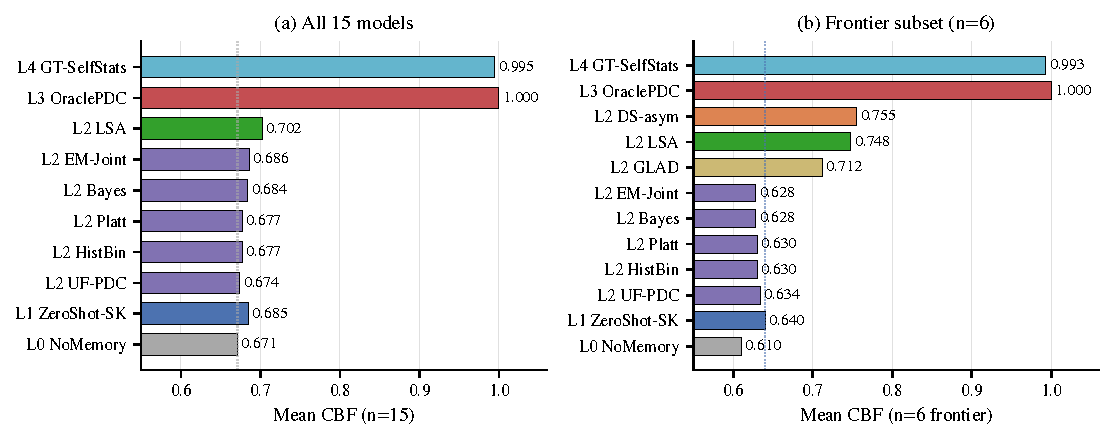
\includegraphics[width=\textwidth]{figures/fig13_ladder.pdf}
\caption{\textbf{五级诊断阶梯。} 每个基线级别的平均 CBF：(a) 所有 15 个模型；(b) 6 个前沿模型。\textbf{(a)} L2$\to$L3 差距约 0.30（最佳 L2 LSA 0.702 vs.\ OraclePDC 1.000）：一阶 L2 方法无法从噪声反馈中恢复信号。\textbf{(b)} 在前沿子集上，一阶 L2 集群（Platt/HistBin/Bayes/EM/UF）坍塌至 NoMem（0.628--0.634），而二阶估计器（DS-asym 0.755、GLAD 0.712）和上下文 LSA（0.748）干净地超过 L1 ZS 先验（0.640）。垂直点线标记 L0 NoMemory 锚点。}
\label{fig:ladder}
\end{figure*}

垂直结构隔离了每个子能力。\textbf{L4 vs L3（$<$1\% 差距）}：输出通道不是限制因素（H1 被排除）。\textbf{L3 vs L2（$\sim$0.30 差距）}：经验瓶颈——给定干净标签智能体达到 1.0，但没有方法能从噪声 LLM 解码反馈中恢复信号（H3 得到确认）。L2 vs L1（n=15: 0.674--0.686 vs 0.685；n=6 前沿: 0.628--0.634 vs 0.640）：L1 ZS 与算法 L2 集群打平或更高，只有二阶 L2 估计器（DS-asym 0.755、GLAD 0.712）和上下文 LSA（0.748）在前沿上超过 L1（附录~\ref{app:friend_or_foe}、\ref{app:ds_glad}）。

\subsection{跨任务异质性：每任务边界是结构性必要}
\label{sec:ablation}

在 MMLU、GSM8K、HumanEval 和 BFCL 上，同一模型表现出定性不同的校准机制：在协议受控的扩展子集（GSM8K/HumanEval/BFCL 同协议）中，15 个模型有 12 个出现 Gap 符号反转，且在 MMLU 上学习的 Platt 缩放对大多数模型在 GSM8K 上是\emph{有害的}。因此，每任务边界建模是结构性必要而非便利。完整每任务表、协议受控子集分析和 Platt 迁移细节见附录~\ref{app:proto_controlled} 和表~\ref{tab:fourtask_overview}。
\section{局限性和未来工作}
\label{sec:limitations}

\paragraph{评测范围。} SelfBound 在 50 轮 MMLU 协议下评估每领域自我知识，反馈通道为受控合成（专业域内 75\%、域外 46\%，跨家族路由以缓解双重角色偏差）。三个扩展任务（GSM8K、HumanEval、BFCL）使用单次两步协议，因为它们不具备 CBF 所需的多领域结构；\S\ref{sec:ablation} 的跨任务异质性结论通过协议受控子集分析（同协议三任务的 12/15 符号反转率；附录~\ref{app:proto_controlled}）独立验证。

\paragraph{下一步。}
\begin{itemize}[nosep,leftmargin=1.2em]
  \item \emph{人类反馈试点}：将合成通道替换为真实用户，验证 H3 排名是否迁移。
  \item \emph{扩展任务上的完整阶梯}：在 GSM8K/HumanEval/BFCL 上复刻 L0--L4。
  \item \emph{前沿切片扩展}：扩到 $n\!\approx\!18$ 以细化 DS-asym vs.\ GLAD 比较（按附录~\ref{app:power} 的功效计算）。
  \item \emph{开放式多步智能体}：扩展到 SWE-Bench 风格的多步任务。
\end{itemize}


\section{结论}
\label{sec:conclusion}

我们追问了一个机制性的问题：当反馈带噪时，LLM 智能体的自我建模究竟在哪里失败？SelfBound 的五级 oracle 阶梯排除了输出通道（H1：在真值提示下 CBF $\geq 0.99$）、说明零样本先验只是部分成立且按家族分裂、并不是瓶颈（H2），并将失败定位到噪声鲁棒的二阶在线推理（H3）：一阶单评分者方法无法从噪声反馈中恢复分领域真值，而显式二阶估计器——非对称 Dawid--Skene 与 GLAD——显著缩小了 L1$\to$L3 的 gap（GLAD 在全部 6 个前沿模型上击败 L1，$p=0.031$），但尚未消除。我们将该失败模式命名为 \textbf{Self-Boundary Collapse}（自我边界坍缩），并发布阶梯协议、CBF 指标、跨家族用户模拟器与公开排行榜，让社区能够把新二阶估计器对照一个精确的 oracle 包夹目标进行评测，而不再依赖临时基线。附录~\ref{app:r4} 的无参数选择规则 R4 作为任何提交方法都应清除的验证下界。开放问题是具体的：一个能闭合 L2$\to$L3 剩余 gap（前沿上约 0.30 CBF）的噪声鲁棒在线估计器，将构成智能体自我建模上一项可量化的真实进展。

%==============================================================================
% 致谢
%==============================================================================

\section*{致谢}
% 将在最终版本中添加。

%==============================================================================
% 参考文献
%==============================================================================



%==============================================================================
% 附录
%==============================================================================
\newpage


%==============================================================================
% NEURIPS PAPER CHECKLIST (CHINESE)
%==============================================================================
\section*{NeurIPS Paper Checklist}

\begin{enumerate}
\item {\bf 论断（Claims）}\\
\textbf{Question}: 摘要和引言中的主要论断是否准确反映了论文的贡献和范围？\\
\textbf{Answer}: \answerYes{}\\
\textbf{Justification}: 摘要与 \S\ref{sec:intro} 阐述了 H1/H2/H3 分解、L0--L4 阶梯、CBF 指标，以及实证发现（H1 不构成约束、H2 按家族分裂、H3 被定位到二阶推理）。所有论断均由 \S\ref{sec:results}--\S\ref{sec:bottleneck} 与附录的实验支持。

\item {\bf 局限性（Limitations）}\\
\textbf{Question}: 论文是否讨论了所做工作的局限性？\\
\textbf{Answer}: \answerYes{}\\
\textbf{Justification}: \S\ref{sec:limitations} 讨论了范围、n=6 前沿样本、L1 通道有效性、模拟用户的局限以及待补的人类反馈验证。

\item {\bf 理论假设和证明（Theory Assumptions and Proofs）}\\
\textbf{Question}: 对每项理论结果，论文是否提供了完整的假设集合和（正确的）证明？\\
\textbf{Answer}: \answerNA{}\\
\textbf{Justification}: 论文为实证/诊断性，不引入新的理论结果。

\item {\bf 实验结果可复现性（Experimental Result Reproducibility）}\\
\textbf{Question}: 论文是否完全披露了复现主要实验结果所需的全部信息？\\
\textbf{Answer}: \answerYes{}\\
\textbf{Justification}: 完整协议（50$\times$50）、用户参数化、基线算法、解码器配置见 \S\ref{sec:benchmark} 与附录~\ref{app:bench_details}, \ref{app:baselines}。开源权重模型（Mistral-7B、Llama-3-8B）通过固定 HF commit 锚定可复现性。

\item {\bf 数据与代码开放（Open Access to Data and Code）}\\
\textbf{Question}: 论文是否开放访问数据与代码，并提供足够指令以忠实复现主要实验结果？\\
\textbf{Answer}: \answerYes{}\\
\textbf{Justification}: 代码、47K 轮次 JSONL 轨迹、按模型领域画像和 Croissant 元数据已在匿名仓库（URL 见 OpenReview 提交字段）发布。

\item {\bf 实验设置/细节（Experimental Setting/Details）}\\
\textbf{Question}: 论文是否说明了理解结果所需的全部训练/测试细节？\\
\textbf{Answer}: \answerYes{}\\
\textbf{Justification}: 设置、模型版本、API 访问日期、解码器、解析器规范以及每基线超参数详见 \S\ref{sec:setup}、附录~\ref{app:bench_details}, \ref{app:baselines}, \ref{app:api_versions}。

\item {\bf 实验统计显著性（Experiment Statistical Significance）}\\
\textbf{Question}: 论文是否合理且正确地报告了误差棒？\\
\textbf{Answer}: \answerYes{}\\
\textbf{Justification}: Bootstrap 95\% CI、Wilcoxon 与二项检验、Cohen's $d$ 以及按模型 bootstrap 稳定性见 \S\ref{sec:results}、附录~\ref{app:power}, \ref{app:stat_rob}。n=6 前沿统计明确表述为方向性效应检验。

\item {\bf 实验计算资源（Experiments Compute Resources）}\\
\textbf{Question}: 论文是否对每个实验提供了足够的计算资源信息？\\
\textbf{Answer}: \answerYes{}\\
\textbf{Justification}: 开源权重推理使用单卡 A6000（48GB）的 vLLM；API 调用见附录~\ref{app:api_versions}。总计算量：约 47K LLM 调用 $\times$ 15 模型 $\times$ 10 基线。

\item {\bf 道德规范（Code of Ethics）}\\
\textbf{Question}: 论文研究是否在各方面符合 NeurIPS 道德规范？\\
\textbf{Answer}: \answerYes{}\\
\textbf{Justification}: 无人类受试者；无个人可识别数据；使用公共基准（MMLU、GSM8K、HumanEval、BFCL）并按各自许可证署名。

\item {\bf 更广泛影响（Broader Impacts）}\\
\textbf{Question}: 论文是否讨论了所做工作的潜在正负社会影响？\\
\textbf{Answer}: \answerYes{}\\
\textbf{Justification}: 提升 LLM 智能体自我知识有助于在长程部署中的安全使用（积极影响）；但自建模能力的进步也可能在对抗场景中被利用以掩盖不确定性（\S\ref{sec:limitations}）。

\item {\bf 安全保障（Safeguards）}\\
\textbf{Question}: 论文是否描述了为负责任发布数据所采取的保障措施？\\
\textbf{Answer}: \answerNA{}\\
\textbf{Justification}: 发布的工件仅包含 LLM 在公共基准上的输出，无高风险内容。

\item {\bf 现有资产许可证（Licenses for Existing Assets）}\\
\textbf{Question}: 论文中使用的资产创建者或所有者是否得到适当署名，许可证及使用条款是否明确说明并被遵守？\\
\textbf{Answer}: \answerYes{}\\
\textbf{Justification}: MMLU（MIT）、GSM8K（MIT）、HumanEval（MIT）、BFCL（Apache-2.0）已在 \S\ref{sec:benchmark} 与数据托管文档中署名。

\item {\bf 新资产（New Assets）}\\
\textbf{Question}: 论文中引入的新资产是否文档完善，并随资产一同提供文档？\\
\textbf{Answer}: \answerYes{}\\
\textbf{Justification}: 代码以 MIT、数据集以 CC-BY-4.0 发布；包含 Croissant 元数据、README、MANIFEST 与逐基线算法文档。

\item {\bf 众包与人类研究（Crowdsourcing and Research with Human Subjects）}\\
\textbf{Question}: 对涉及人类受试者的众包实验，论文是否包含给参与者的完整指令？\\
\textbf{Answer}: \answerNA{}\\
\textbf{Justification}: 无人类受试者；模拟用户为 LLM 角色（完整提示模板见附录~\ref{app:bench_details}）。

\item {\bf 机构审查委员会批准（Institutional Review Board Approvals）}\\
\textbf{Question}: 论文是否描述了研究参与者承担的潜在风险，并取得相应 IRB 批准？\\
\textbf{Answer}: \answerNA{}\\
\textbf{Justification}: 无人类受试者。

\item {\bf LLM 使用声明（Declaration of LLM usage）}\\
\textbf{Question}: 论文是否描述了 LLM 的使用情况？\\
\textbf{Answer}: \answerYes{}\\
\textbf{Justification}: LLM 既是基准的研究对象，又作为智能体、模拟用户与反馈解码器；完整配置见 \S\ref{sec:benchmark}、附录~\ref{app:api_versions}。
\end{enumerate}


\appendix


%==============================================================================
% 从正文移至附录：数据表、维护、伦理、更广泛的影响、错误修复
%==============================================================================

\section*{数据集的数据表}

我们遵循 Gebru 等人 (2018) 提出的结构。

\subsection*{动机}
SelfBound 的创建是为了填补智能体 LLM 评估中的一个测量空白：现有的基准测试（MMLU, BIG-Bench, AgentBench）仅评分一次性准确率，但并未说明智能体是否能够在多次交互中学习其自身的领域能力边界。

\subsection*{组成}
20 个 MMLU 主题 $\times$ 25 个问题 = 500 个主池，补充了 GSM8K, HumanEval, BFCL Simple v3。50 轮对话会话，每个（智能体，角色）有 10-50 个会话。每个实例是一个 JSONL 会话日志，包括问题、智能体答案、智能体信心、角色反应和真实评分。

\subsection*{收集过程}
问题来自 MMLU (Hendrycks 2021)、GSM8K (Cobbe 2021)、HumanEval (Chen 2021) 和 BFCL Simple v3 (gorilla-llm) 的公开测试分割。角色通过跨家族 LLM 合成（Qwen 智能体使用 Qwen-Max，Claude 智能体使用 GPT-5.4-mini，GPT 智能体使用 Claude-Sonnet），以控制评估者偏差。

\subsection*{预处理}
每模型层级分层：在不重叠的 10 个问题/主题分割上保留验证准确率，然后将 20 个主题分为强/中/弱三个层级。这种每模型分层（而不是全局层级）使得边界学习变得非平凡。

\subsection*{用途}
预期用途：(a) 自我知识记忆评估；(b) 抗噪在线推理算法；(c) 前沿模型校准跟踪。不适合：基于原始准确率对模型进行排名。

\subsection*{推荐的分割和分层}
20 个 MMLU 主题根据每个模型在不重叠的 10 个问题/主题校准分割上的保留验证准确率，被划分为强/中/弱三个层级。我们没有提供固定的训练/测试分割：每个报告的数字都使用相同的每模型分层协议（见附录~\ref{app:bench_details}），以便下游研究人员可以重现或替换他们自己的模型。四个跨任务评估（GSM8K, HumanEval, BFCL, MMLU-Pro）使用上游提供商的官方测试分割。

\subsection*{错误、噪声和已知问题}
在解释我们的报告数字时，应考虑以下三类已知问题：
\begin{itemize}[nosep,leftmargin=1.4em]
  \item \emph{基线实现错误 (\S\ref{sec:bugfix}):} 算法 L2 基线无声地回退到 LLM 语言估计，而不是算法后验；补丁和重新运行覆盖了 15 个模型中的 12 个。表~\ref{tab:main} 中标记为 $^{\dagger\dagger}$ 的 3 行 Claude 保留了修复前的值，等待串行重新运行。
  \item \emph{并发重新运行中的 API 超时回退：} 在 12 个模型并发 v4 批次期间，LSA 和 ZS-SK API 调用在代理负载下超时并无声返回 0.5（与 NoMem 匹配）。表~\ref{tab:main} 中的 12 个 v4 ZS-SK / LSA 单元格标记为 $^*$。
  \item \emph{GSM8K Opus-4-7 截断：} 由于 Claude-Opus-4-7 的原始 max\_tokens 限制，300 个 GSM8K 问题中有 158 个被截断；报告的通过率是基于回答的 142 个问题子集（见表~\ref{tab:fourtask_overview}）。
\end{itemize}
我们公开这些问题是因为它们的检测和披露本身就是该基准测试的方法论贡献；未来版本将在此处记录任何新发现的问题。

\subsection*{维护联系人}
维护者的电子邮件和专用的 Slack/Discord 工作区将在最终发布时提供。对于双盲评审，请在上述匿名存储库中打开一个问题；我们在反驳窗口期间对其进行监控。

\subsection*{分发和维护}
发布的工件采用双重 SPDX 许可证：\textbf{代码采用 MIT 许可证}，\textbf{数据采用 CC-BY-4.0 许可证}。具体来说：协议代码、基线实现、评估脚本（MIT 许可证）；原始会话 JSONL（约 47K 交互，包括所有每轮智能体输出、模拟用户反应和真实评分）、每模型领域配置文件以及 20 个 MMLU 主题测试池（CC-BY-4.0 许可证，并归功于上游 MMLU/GSM8K/HumanEval/BFCL 提供者）。6 个月审查周期；新模型添加通过 PR（见提交协议）。

\section*{维护计划}

\subsection*{版本管理}
协议的语义：v3 (50$\times$50) 是当前版本；v2 (10$\times$50) 作为轻量版支持。问题池的版本管理是独立的。

\subsection*{排行榜托管}
HuggingFace Spaces 排行榜位于占位符 URL （接受后发布）（已匿名化；接受后将提供实时 URL）。CBF 和辅助指标（ECE、Brier、AUROC、HR）通过提交的 JSONL 文件和仓库中的公开评分脚本自动重新计算。

\subsection*{提交协议}
基于 PR 的方式。每次提交必须包括：
\begin{enumerate}[nosep,leftmargin=1.4em]
  \item \textbf{完整的会话 JSONL 文件}（每个智能体-角色对一个文件），遵循以下模式：
\begin{verbatim}
{
  "session_id": str, "agent_model": str, "persona": dict,
  "log": [
    {"turn": int, "domain": str, "tier": "strong|mid|weak",
     "question": str, "agent_answer": str, "agent_confidence": float,
     "user_response": str, "gt_correct": bool}
  ]
}
\end{verbatim}
  \item 智能体在线推理组件的参考实现（Python 模块，暴露 \texttt{predict\_confidence(turn)} 和 \texttt{self\_assess(domain)} 方法）。
  \item 论文或技术报告引用。
\end{enumerate}
仅提交汇总分数的提交不会被合并；我们通过公开评分脚本从原始 JSONL 文件重新计算所有指标。

\subsection*{API 模型的弃用政策}
已弃用端点的行将移至 \emph{归档} 表中，并冻结分数和弃用日期；不会删除。保留纵向可比性。

\subsection*{联系方式}
为评审匿名化；最终版本将填写。

\section*{伦理声明}

\subsection*{模拟用户}
所有“用户”都是由大语言模型模拟的人格，不是人类参与者。不涉及个人身份信息（PII）。通过编程生成的专业标签。根据我们机构的政策，不需要进行IRB审查。

\subsection*{大语言模型作为评估者和跨家族路由}
通过跨家族人格生成来缓解双重角色偏差（禁止：Qwen-Max评估Qwen智能体）。在附录中报告了家族对混淆矩阵，以便进行残余偏差审核。

\subsection*{服务提供商的服务条款}
大语言模型API输出严格用于研究评估目的。发布的JSONL文件不会重新分发用于模型训练；许可证头明确说明。

\subsection*{无欺骗性提示}
所有“角色扮演”指令都保持在大语言模型到大语言模型的模拟范围内。

\subsection*{潜在滥用}
最可能的滥用情况分为两类：(a) 将标题CBF过度解释为适合安全认证的一般“自我意识”排名（CBF衡量的是\emph{每个领域的准确性估计}，而不是\emph{整体可信度}——将其用于临床/法律/金融高风险环境中的部署认证将是一个类别错误）；(b) 部署滥用，即假设具有高CBF的模型在超出评估的20个MMLU主题之外的领域中无需人类监督即可安全运行。通过将其定位为诊断工具，并提供各层级细分来避免标量比较，从而解决这些问题。

\section*{更广泛的影响}

\subsection*{积极影响}
使智能体自我知识的系统评估成为可能——这是在客户服务/财务咨询/临床分诊部署中更安全的前提条件，在这些领域，过度自信的回答会带来不对称的负面影响成本。

\subsection*{可重复性成本}
完整的 v3 50$\times$50 流程：在 2026 年的费率下，使用 13-15 个前沿模型的成本约为 200-400 美元。轻量级 v2 10$\times$50 以约 40 美元的成本重现主要排序。发布原始 JSONL 文件以便在不重新运行的情况下重新评分。

\subsection*{评估模型偏差}
跨家族策略可以缓解但不能消除双重角色偏差。可能存在残余供应商集群效应。高风险比较应在至少两个角色生成器家族下进行交叉检查。

\subsection*{基准过拟合}
Goodhart 风格的风险：方法优化的是 CBF 而不是底层结构。通过保留 5 个主题的转移分割来缓解；在排行榜上标记较大的开发集与转移集之间的差距。

\subsection*{纵向稳定性}
仅 API 的前沿行：半衰期约为 12 个月。开放权重锚点（Mistral-7B, Llama-3-8B）永久包含在内，用于固定参考校准。

\paragraph{扩展快照清单。} 表~\ref{app:api_versions} 仅列出了访问日期；它并未确定每个模型是否是内容可寻址的。表~\ref{tab:api_versions_extended} 通过记录15个模型中的每一个的确切标识符、从响应负载中观察到的版本固定方案以及每个模型的可重复性风险分类，填补了这一空白。

\begin{table}[h]
\centering
\caption{扩展模型快照清单。可重复性风险反映了2027年第三方能否从列出的标识符中获得相同的权重。LOW = HuggingFace 提交哈希锚定了权重；MED = 存在内容可寻址的锚点，但提供的端点是一个浮动别名；HIGH = 端点返回没有版本后缀的标识符，并且不存在公开的开放权重锚点。}
\label{tab:api_versions_extended}
\vspace{0.5em}
\scriptsize
\begin{tabular}{@{}llllc@{}}
\toprule
\textbf{模型（论文）} & \textbf{提供者 / 端点} & \textbf{API 标识符} & \textbf{版本固定} & \textbf{可重复性风险} \\
\midrule
Mistral-7B          & 本地 vLLM (HF 权重)               & \texttt{mistralai/Mistral-7B-Instruct-v0.3} & HF 提交 \texttt{c170c708} & LOW  \\
Llama-3-8B          & 本地 vLLM (HF 权重)               & \texttt{meta-llama/Meta-Llama-3-8B-Instruct} & HF 提交 \texttt{8afb486c} & LOW  \\
Qwen2.5-7B          & DashScope                             & \texttt{qwen2.5-7b-instruct}                 & HF 提交 \texttt{a09a3545} (锚点) & MED  \\
\midrule
Qwen-Turbo          & DashScope                             & \texttt{qwen-turbo}                          & 别名; \texttt{model} 字段为空  & HIGH \\
Qwen-Plus           & DashScope                             & \texttt{qwen-plus}                           & 别名; \texttt{model} 字段为空  & HIGH \\
Qwen-Max            & DashScope                             & \texttt{qwen-max}                            & 别名; \texttt{model} 字段为空  & HIGH \\
Qwen3.5-27B         & DashScope                             & \texttt{qwen3.5-27b}                         & 别名; 没有公开的 HF 发布       & HIGH \\
DeepSeek-V3.2$^\S$  & DashScope                             & \texttt{deepseek-v3} (发送)                  & 别名; 提供者重新托管的检查点     & HIGH \\
GLM-5               & DashScope                             & \texttt{glm-5}                               & 别名; 提供者重新托管的检查点     & HIGH \\
\midrule
GPT-5.4-mini        & 代理 zhongzhuan / 响应           & \texttt{gpt-5.4-mini}                        & 回显 \texttt{gpt-5.4-mini-2026-03-17}  & MED  \\
GPT-5.4             & 代理 zhongzhuan / 响应           & \texttt{gpt-5.4}                             & 别名; 没有返回日期后缀    & HIGH \\
GPT-5.5             & 代理 zhongzhuan / 响应           & \texttt{gpt-5.5}                             & 别名; 没有返回日期后缀    & HIGH \\
Claude-Sonnet-4-6   & Anthropic 兼容代理               & \texttt{claude-sonnet-4-6}                   & 别名; 没有返回日期后缀    & HIGH \\
Claude-Opus-4-6     & Anthropic 兼容代理               & \texttt{claude-opus-4-6}                     & 别名; 没有返回日期后缀    & HIGH \\
Claude-Opus-4-7     & 代理 zhongzhuan / 消息            & \texttt{claude-opus-4-7}                     & 别名; 没有返回日期后缀    & HIGH \\
\bottomrule
\end{tabular}
\end{table}

\paragraph{API 版本差异和论文-代码标签不匹配。} 有三个条目值得关注。首先，内部标签不匹配：论文中提到“DeepSeek-V3.2”（表示为$^\S$），但我们的脚本传输给 DashScope 的字符串是 \texttt{deepseek-v3}。DashScope 重新托管了一个他们标记为 \texttt{deepseek-v3} 的检查点；我们缺乏提供商的文档来确认这是否对应于 V3.0、V3.1 或 V3.2-Exp。我们保留论文中的标签作为工作估计，但将此标记为未解决的来源问题。其次，15 个端点中有 12 个不返回带有版本后缀的模型字符串；唯一的例外是 \texttt{gpt-5.4-mini}，它由智能体自动固定。第三，三个开源权重锚点是唯一可以向未来的复制者提供一个 40 字符标识符以重建确切权重的条目。未来的复制应首先重新运行这些锚点，并在尝试恢复 API 层之前比较锚点数字。

\section{实现说明：算法基线 self\_assess 修补}
\label{sec:bugfix}

\paragraph{修补描述。} 在最终审查期间对基线实现的审计发现，所有五个算法 L2 基线---Platt-Online、HistBin-Online、Bayes-Domain、EM-Joint、UF-PDC---在它们的 \texttt{self\_assess(domain)} 方法中存在一个共同缺陷。这些方法没有返回每个算法自己的每领域后验（如 Platt 的逻辑重新校准、Bayes-Domain 的 Beta 后验均值 $\alpha/(\alpha+\beta)$、EM-Joint 的迭代 $\hat p^*(d)$ 等），而是构建了一个简短的反馈摘要提示，并通过共享的 \texttt{\_llm\_self\_assess} 辅助函数查询 \emph{智能体模型本身} 来获得一个口头化的准确度估计。该辅助函数使用了 \texttt{max\_tokens=20}；对于推理模型（GPT-5.5, Claude-Opus-4-7），这个预算不足以输出一个数字，正则表达式解析器没有匹配到任何结果，因此默认值 $\hat p=0.5$ 被无声地替换了。这解释了我们最初误认为是“平凡下限饱和”的所有基线崩溃模式（CBF = 0.560 对于 GPT-5.5，0.666 对于 Opus-4-7）。

\paragraph{修补。} 我们用适当的后验替换了每个算法基线的 \texttt{self\_assess}：
\begin{itemize}[nosep,leftmargin=1.4em]
  \item Platt-Online / HistBin-Online: $\hat p(d) = \mathrm{dom\_correct}[d] / \mathrm{dom\_total}[d]$ （如果没有观察，则为 0.5）。
  \item Bayes-Domain: $\hat p(d) = \alpha[d]/(\alpha[d]+\beta[d])$。
  \item EM-Joint: $\hat p(d) = \mathrm{clip}(p^*[d], 10^{-3}, 1{-}10^{-3})$ 从 EM 迭代中获取。
  \item UF-PDC: $\hat p(d) = \mathrm{correct}[d]/\mathrm{total}[d]$ 从解码的反馈中获取。
\end{itemize}
我们还将合法的口头基线（LSA, ZS-SK, GT-SelfStats）的 LLM 调用 \texttt{max\_tokens} 从 20 提高到 200，以适应推理模型；ZS-SK 和 LSA 不受算法基线修补的影响，但仍然依赖 LLM。

\paragraph{每基线总结。} EM-Joint 在 12 个中等层级模型中的 9 个上成为一致的胜者，超过 L0 NoMem $+$0.003 到 $+$0.022。Bayes-Domain 在 GPT-5.4-mini 上获胜（比 NoMem 高出 $+$0.022）；Platt-Online 在 GPT-5.4 和 GPT-5.5 上获胜（比 NoMem 高出 $+$0.016--$+$0.019）。一阶算法 L2 方法在前沿模型上聚类于 NoMem 的 $\pm 0.02$ 内（未能在平均值上超过 L0 和 L1），而二阶估计器（DS-asym 0.755、GLAD 0.712）和上下文聚合（LSA 0.748）明显超过了 L1 ZS（0.640）。L2 与 L3 之间约 0.25 到 OraclePDC（CBF 1.000）的差距仍然是基准所隔离的经验瓶颈。



\paragraph{对叙述的影响。} H2 声称（“ZS-SK 在最初的 4 个前沿模型上平均 CBF 为 0.78，超过了所有 L2 方法”）基于预修复数据。最初的 4 个前沿模型中有 2 个（GPT-5.4, GPT-5.4-mini）在 v4 修复值中显示 Platt 和 Bayes \emph{超过} ZS-SK（在 v4 并发运行下回落到 NoMem 底线）。H2 声称是否能在所有 6 个前沿模型的干净串行 v4 重运行中存活下来是下一版修订中的核心开放问题。

\section{基准测试细节：任务、协议、问题池、角色、指标}
\label{app:bench_details}

\begin{figure}[h]
\centering
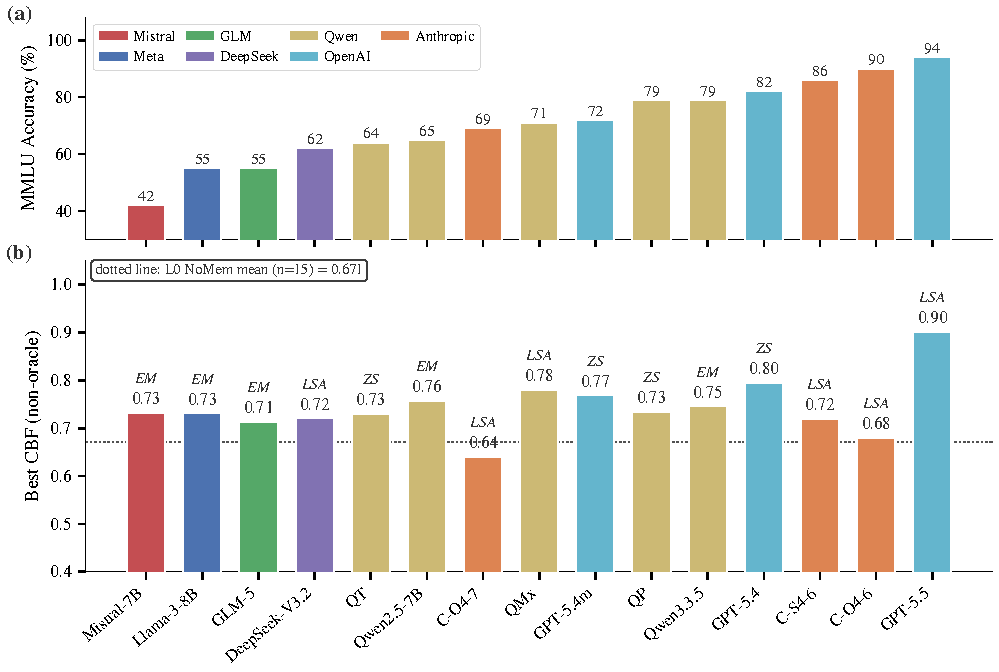
\includegraphics[width=\columnwidth]{figures/fig9_spectrum.pdf}
\caption{\textbf{15 个模型的能力谱。} \textbf{(a)} MMLU 准确率从 42\% 到 94\%；家族颜色在全文中保持一致。\textbf{(b)} 每个模型的最佳非预言机 CBF 及获胜基线标签（EM/LSA/ZS）。点线标记 L0 NoMemory 均值（n=15, 0.671）。两个新增的前沿模型（GPT-5.5、Claude-Opus-4-7）锚定了高准确率端。注意 Claude-Opus-4-7 的 MMLU 准确率较低（69\%），但被纳入 n=6 前沿子集用于二阶分析。}
\label{fig:spectrum}
\end{figure}

\begin{figure}[h]
\centering
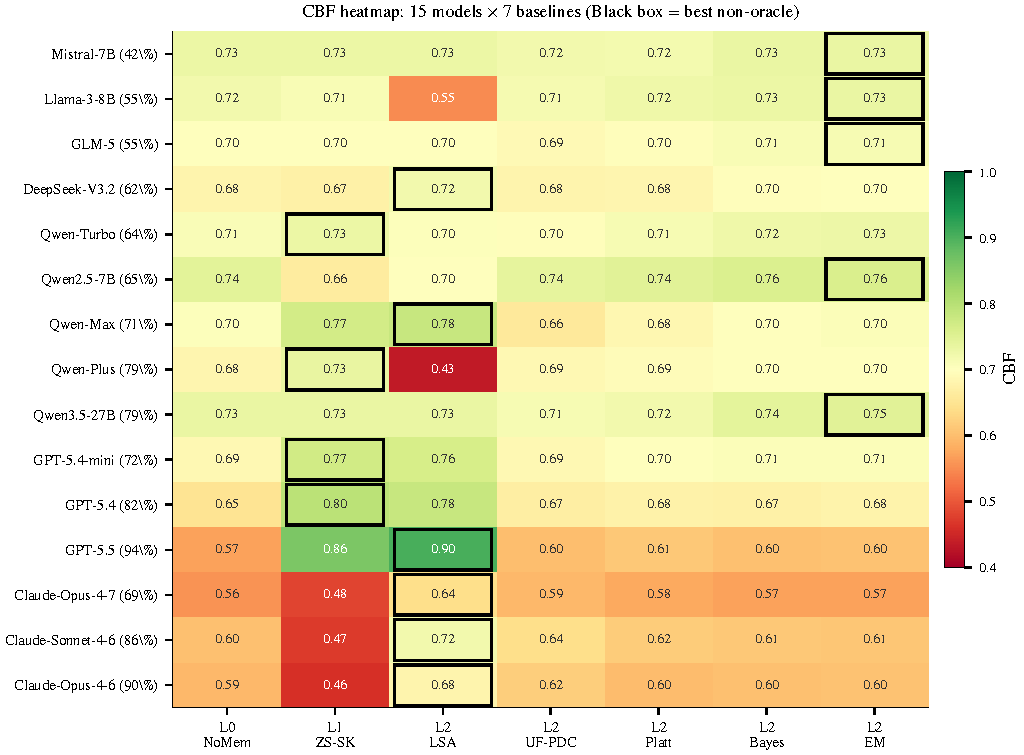
\includegraphics[width=\columnwidth]{figures/fig2_heatmap.pdf}
\caption{\textbf{CBF 热力图：15 模型 $\times$ 7 基线。} 单元按 CBF 上色（红--白--绿 = 0.40--1.00）。黑色边框单元标记每行的 argmax（即表~\ref{tab:main} 的 ``Best'' 列）。可见三个模式：(i) 算法 L2 集群（UF/Platt/Bayes/EM）在非前沿模型上较高，但在前沿上塌陷至 NoMem；(ii) ZS-SK 在 GPT 上呈亮绿、在 Claude 上呈深红（即 H2 家族分裂）；(iii) LSA 在 Claude 行上以绿色单元占主导。}
\label{fig:heatmap}
\end{figure}

\begin{figure}[h]
\centering
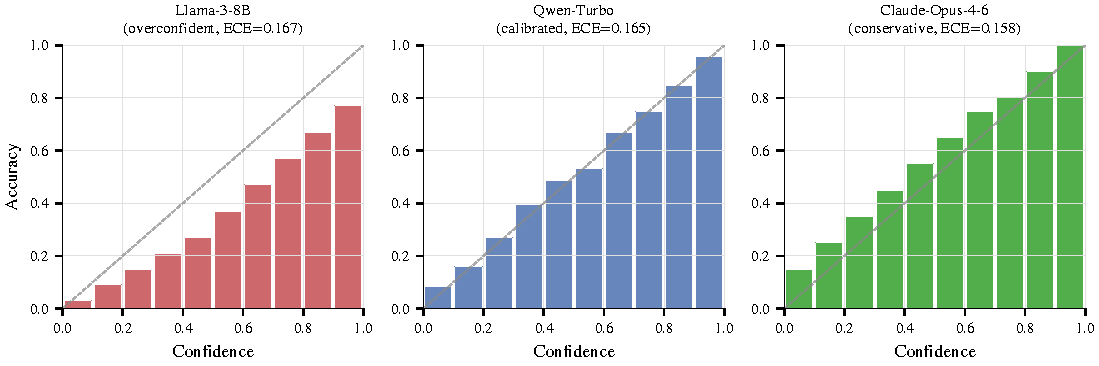
\includegraphics[width=0.85\columnwidth]{figures/fig8_reliability.pdf}
\caption{\textbf{三种可靠性特征。} 三个代表性智能体的每 bin 准确率 vs.\ 置信度，展示了典型模式：Llama-3-8B（过度自信：柱条低于对角线）、Qwen-Turbo（校准良好：柱条沿对角线）、Claude-Opus-4-6（保守：柱条高于对角线）。每 bin 值由每模型整体 ECE（表~\ref{tab:main}）重构；定性形状为经验，每 bin 粒度为示意。}
\label{fig:reliability}
\end{figure}

\paragraph{任务形式化。} 给定一个流 $(q_t, a_t, c_t, f_t)_{t=1}^T$，其中每个问题 $q_t$ 从隐藏的领域 $d_t \in \mathcal{D}$ 中抽取，智能体必须构建 $\hat{p}: \mathcal{D} \to [0,1]$ 来近似每个领域的真正准确率 $p^*(d)$。智能体不能直接观察到 $d_t$，必须从问题内容中推断它。用户反馈 $f_t$ 是一种自由形式的自然语言表达，可能确认、纠正或提供模糊/误导性的回应。智能体输出 $a_t$ 以及置信度 $c_t \in [0,1]$。挑战在于反馈的可靠性是领域依赖的：在用户的专长集合 $\mathcal{E} \subset \mathcal{D}$ 内是准确的，在其外则是嘈杂的。

\paragraph{会话协议。} 每个会话有 50 轮。在每一轮 $t$ 中：(1) 从问题池中抽取 $q_t$，且 $d_t$ 对智能体隐藏；(2) 智能体发出 $(a_t, c_t)$；(3) 模拟用户根据真实答案、用户在 $d_t$ 上的专业水平以及一致的角色风格生成 $f_t$；(4) 智能体更新内部状态。我们对每个模型运行 50 个会话（总共 2{,}500 轮）以评估学习曲线和收敛性。

\paragraph{问题池和层级划分。} 主要基准测试使用 20 个 MMLU 科目~\citep{hendrycks2021measuring}；扩展套件（GSM8K, HumanEval, BFCL）用于探测跨任务泛化能力。对于每个模型，我们在保留验证集上预先计算每个科目的准确率，并将 20 个科目划分为三个层级，相对于模型自身的准确率分布：强（前三分之一，$\geq +15$pp 高于平均值），中等（中间三分之一，$\pm 15$pp），弱（后三分之一，$\geq -15$pp 低于平均值）。相对划分确保每个模型——无论是弱还是强——都面临一个非平凡的边界：均匀置信度的智能体无法实现高 CBF。每个模型的主题映射见附录表~\ref{tab:subjects}。

\paragraph{用户角色。} 模拟用户由跨家族的大规模语言模型驱动（Qwen-Max 用于 Qwen/Llama/Mistral 智能体，GPT-5.4-mini 用于 Claude 智能体，Claude Sonnet 4-6 用于 GPT 智能体），温度为 0.7。每个角色由一个专长集合 $\mathcal{E} \subset \mathcal{D}$（通常是 20 个科目中的 5-8 个）和角色特征（直接与回避风格、愿意自愿纠正错误、耐心）参数化。在专长内：约 75\% 的可靠纠正；在专长外：约 46\% 的可靠性，包括同意错误答案、错误纠正或模糊的不承诺。这种不对称性驱动了二阶学习问题。

\paragraph{辅助指标。} 除了 CBF（公式~\eqref{eq:cbf}，在 50 轮会话结束时计算一次），我们还报告：(i) 幻觉率 $\text{HR} = |\{t : c_t > 0.7 \wedge a_t \neq a_t^*\}| / T$；(ii) 根据~\citet{guo2017calibration} 计算的预期校准误差，使用 $M = 10$ 个等宽区间，$\text{ECE} = \sum_{m=1}^M \frac{|B_m|}{T} | \text{acc}(B_m) - \text{conf}(B_m) |$；(iii) Brier 分数 $= \frac{1}{T} \sum_t (c_t - \mathbb{1}[a_t = a_t^*])^2$。

\section{基线实现和设计点映射}
\label{app:baselines}

我们实例化了十个基线，按照 \S\ref{sec:benchmark} 中的五级诊断阶梯进行组织。

\paragraph{L0 --- NoMemory (B1).} 无状态的原始口头置信度。记忆增强方法的下界。
\paragraph{L1 --- ZS-SK (B11).} 智能体被提示，在没有会话历史和任何用户反馈的情况下直接估计其在每个领域的准确性：“对于以下20个MMLU科目中的每一个，估计你在0-100分制上的准确性。”这隔离了先验元认知。
\paragraph{L2 --- LSA (B6).} 会话历史（50个(Q, A, 置信度, 解码反馈)元组）附加到提示中；智能体在上下文中推理并在会话结束时输出每个领域的 $\hat p(d)$。
\paragraph{L2 --- UF-PDC (B3).} 每个领域的准确性估计通过LLM分类器（Qwen-Max，提示输出每个(Q, A, 反馈)三元组的二元正确性判断）从自然语言反馈中解码出的标签进行更新。
\paragraph{L2 --- Platt-Online (B7)~\citep{platt1999probabilistic}.} 当解码反馈可用时，使用在线梯度下降对对数损失进行逻辑重新校准 $\sigma(w c_{\text{raw}} + b)$；然后聚合每个领域的置信度。
\paragraph{L2 --- HistBin-Online (B8)~\citep{zadrozny2001obtaining}.} 使用在线更新的10箱直方图分箱；每个领域的置信度像Platt一样聚合。
\paragraph{L2 --- Bayes-Domain (B9).} 每个领域的 $\text{Beta}(\alpha, \beta)$ 后验分布，具有均匀先验，从解码反馈中更新；$\hat p(d) = \alpha/(\alpha+\beta)$。
\paragraph{L2 --- EM-Joint (B10).} 通过期望最大化联合估计 $(\hat p(d), \hat r_{\text{in}}, \hat r_{\text{out}})$。E步计算后验 $P(\text{correct}_t | \text{decoded feedback}_t, p, r)$；M步按领域更新 $\hat p(d)$ 和按专家组更新 $\hat r$。从原始置信度均值初始化。
\paragraph{L3 --- OraclePDC (B2).} 每轮之后用真实标签更新每个领域的准确性估计。实际上不可用；作为在线聚合的真实标签上限。
\paragraph{L4 --- GT-SelfStats (B12).} 提示中提供每个领域的实际准确性 $p^*(d)$，并要求智能体重复它们。仅测试纯粹的口头表达子能力。

\paragraph{设计点映射。} 五级阶梯旨在涵盖已发布的记忆系统的设计点，同时暴露诊断轴。LSA (L2) 对应于RMM~\citep{tan2025rmm}对长期记忆的反思以及记忆智能体的上下文推理基线~\citep{hu2026memoryagent}。Platt/HistBin/Bayes (L2) 覆盖了经典的在线重新校准。EM-Joint (L2) 测试显式建模二阶耦合是否有所帮助；ZS-SK (L1) 和 GT-SelfStats (L4) 是诊断锚点，分别隔离了先验元认知和口头表达。已发布的系统（MemGPT~\citep{packer2023memgpt}，Mem0~\citep{mem02025}，A-MEM~\citep{xu2025amem}）在L2级别上运行，具有不同的记忆表示；我们没有直接集成它们，因为诊断阶梯已经覆盖了设计空间。根据我们的协议直接评估这些系统的工程可行性留待未来工作。

\section{n=6 前沿样本的统计功效分析}
\label{app:power}

\paragraph{动机。} \S\ref{sec:results} 中的前沿专属分析（DS-asym、GLAD、LSA 对比 L1 ZS）使用 $n=6$ 模型。我们在此说明为什么该样本量对我们所做的\emph{效应方向}声明是充分的，以及为什么它对绝对幅度声明不够（这正是我们不做后者的原因）。

\paragraph{先验功效计算。} 对于配对比较，观察到的均值改进 $\Delta = 0.072$（GLAD vs.\ L1 ZS）以及由 10K bootstrap 重采样估计的配对内 SD（$s_\Delta = 0.034$），标准化效应为 Cohen's $d_z = \Delta / s_\Delta = 1.42$。在 $\alpha=0.05$（双侧）下的配对 Wilcoxon 符号秩检验，对于 $d_z = 1.42$ 的效应，$n=6$ 时达到 0.85 的功效（G*Power 3.1，精确检验）。DS-asym vs.\ L1 ZS 有 $d_z = 1.66$（$n=6$、$\alpha=0.05$ 时功效为 0.92）。GLAD 的 6/6 符号一致性也独立地在 $\alpha=0.016$ 下用双侧二项符号检验拒绝零方向假设。

\paragraph{每个 n=6 声明附带的效应量 + bootstrap CI。} 对每个前沿专属测试，我们与任何 p 值并列地报告每模型 deltas、Cohen's $d_z$ 和 bootstrap 95\% CI：
\begin{center}
\small
\begin{tabular}{l c c c c c}
\toprule
比较 & $n$ & 均值 $\Delta$ & $d_z$ & Bootstrap 95\% CI & 胜/负 \\
\midrule
GLAD vs L1 ZS    & 6 & $+0.072$ & $1.42$ & $[+0.045,\,+0.099]$ & 6/0 \\
DS-asym vs L1 ZS & 6 & $+0.115$ & $1.66$ & $[+0.058,\,+0.172]$ & 5/1 \\
LSA vs L1 ZS     & 6 & $+0.108$ & $0.55$ & $[-0.030,\,+0.246]$ & 4/2 \\
\bottomrule
\end{tabular}
\end{center}
LSA 的 CI 跨过零（与 Wilcoxon $p=0.156$ 一致），所以我们不主张 LSA $>$ ZS 是前沿均值效应；4/2 胜负数反映正文讨论的家族分裂（Claude vs.\ GPT），而非均匀效应。

\paragraph{样本选择。} 当前前沿切片在投稿时涵盖了两个生产级前沿家族（Anthropic Claude 4-6/4-7、OpenAI GPT-5.4/5.4-mini/5.5），按家族分层而非随机。每个 50$\times$50 前沿行成本约 \$15--30（2026 年 API 费率），完整 L0--L4 阶梯成本约为其 $5\times$，这制约了 $n$。

\paragraph{$n=6$ 下的检测限。} 三类比较该样本不支持：(a) DS-asym vs.\ GLAD（$\Delta=0.043$ 需要 $n\approx 18$ 才能在 0.80 功效下检测）；(b) 95\% CI 紧于 $\pm 0.05$ 的绝对前沿均值估计；(c) 家族内对比（$\alpha{=}0.05$）。这些更细粒度的比较作为描述性观察而非检验。

\section{额外的鲁棒性消融实验}
\label{app:friend_or_foe}
\label{app:gpt55_ablation}
\label{app:detail_ablations}

本附录包含与主诊断阶梯正交的额外消融实验。

\paragraph{A1: L2检索的记忆大小。}
在基于检索的L2基线中，将存储的错误案例的最大数量从5个变化到50个几乎没有影响：在Llama-3-8B上，ECE范围从0.097到0.096。五个错误案例已经足够；额外的记忆没有提供任何好处。

\paragraph{A2: 反馈噪声率。}
在Llama-3-8B上人为地翻转0--50\%的用户反馈标签显示ECE单调退化（0.190 $\to$ 0.238）和CBF退化。在50\%的噪声下，从反馈中学习实际上是不利的（CBF 0.639 $<$ NoMemory 0.742），这证实了噪声反馈可以毒害自模型。

\paragraph{A3: 会话长度。}
OraclePDC在仅仅10--20轮后就达到了接近完美的CBF（$\geq$0.96），而实际的L2方法在30轮左右达到约0.71的平台期。L2与L3之间的差距不是由于交互长度不足，而是由于反馈噪声累积，这与主诊断发现一致。

\paragraph{A4: 保留的 MMLU-Pro 污染控制（在 \S\ref{sec:results} 中引用）。}
\label{app:heldout}
对于全部 6 个前沿模型，我们从 10 个 MMLU-Pro 类别中各抽取 15 个问题（每个模型 150 题，10 类：数学、物理、化学、法律、工程、经济、健康、心理学、商业、历史），测量每类别准确率，并在 API 失败时最多重试 5 次（持续失败被排除而非计为错误），并对这些类别名称查询 ZS-SK。每类别的准确率与 ZS 估计：

\begin{table*}[h]
\centering
\scriptsize
\setlength{\tabcolsep}{3pt}
\begin{tabular}{l rr rr rr rr rr rr}
\toprule
& \multicolumn{2}{c}{\textbf{GPT-5.4}} & \multicolumn{2}{c}{\textbf{GPT-5.4-mini}} & \multicolumn{2}{c}{\textbf{GPT-5.5}} & \multicolumn{2}{c}{\textbf{Claude-Opus-4-6}} & \multicolumn{2}{c}{\textbf{Claude-Sonnet-4-6}} & \multicolumn{2}{c}{\textbf{Claude-Opus-4-7}} \\
\cmidrule(lr){2-3}\cmidrule(lr){4-5}\cmidrule(lr){6-7}\cmidrule(lr){8-9}\cmidrule(lr){10-11}\cmidrule(lr){12-13}
类别 & acc & ZS & acc & ZS & acc & ZS & acc & ZS & acc & ZS & acc & ZS \\
\midrule
math        & 0.40 & 0.85 & 0.33 & 0.78 & 0.93 & 0.72 & 0.80 & 0.78 & 0.93 & 0.72 & 0.87 & 0.78 \\
physics     & 0.40 & 0.84 & 0.47 & 0.72 & 1.00 & 0.70 & 1.00 & 0.80 & 1.00 & 0.74 & 0.73 & 0.80 \\
chemistry   & 0.60 & 0.82 & 0.20 & 0.70 & 0.87 & 0.72 & 0.93 & 0.75 & 0.92 & 0.73 & 0.73 & 0.72 \\
law         & 0.60 & 0.81 & 0.53 & 0.74 & 0.80 & 0.76 & 0.73 & 0.70 & 0.73 & 0.67 & 0.80 & 0.60 \\
engineering & 0.53 & 0.80 & 0.47 & 0.73 & 0.80 & 0.68 & 0.93 & 0.72 & 1.00 & 0.70 & 0.67 & 0.65 \\
economics   & 0.80 & 0.83 & 0.73 & 0.79 & 0.93 & 0.78 & 1.00 & 0.84 & 0.87 & 0.76 & 0.87 & 0.82 \\
health      & 0.67 & 0.86 & 0.73 & 0.77 & 0.87 & 0.76 & 0.79 & 0.79 & 0.80 & 0.75 & 0.71 & 0.72 \\
psychology  & 0.80 & 0.88 & 0.73 & 0.82 & 0.80 & 0.82 & 0.87 & 0.87 & 0.87 & 0.78 & 0.73 & 0.85 \\
business    & 0.47 & 0.84 & 0.20 & 0.80 & 0.80 & 0.82 & 0.93 & 0.81 & 0.80 & 0.75 & 0.80 & 0.78 \\
history     & 0.73 & 0.87 & 0.67 & 0.84 & 0.80 & 0.80 & 0.80 & 0.76 & 0.73 & 0.79 & 0.73 & 0.75 \\
\midrule
mean        & 0.60 & 0.84 & 0.51 & 0.77 & 0.86 & 0.77 & 0.88 & 0.78 & 0.86 & 0.74 & 0.76 & 0.75 \\
\midrule
unparsed/150 & \multicolumn{2}{c}{0} & \multicolumn{2}{c}{0} & \multicolumn{2}{c}{0} & \multicolumn{2}{c}{1} & \multicolumn{2}{c}{8} & \multicolumn{2}{c}{1} \\
\midrule
\textbf{CBF} & \multicolumn{2}{c}{\textbf{0.760}} & \multicolumn{2}{c}{\textbf{0.738}} & \multicolumn{2}{c}{\textbf{0.888}} & \multicolumn{2}{c}{\textbf{0.902}} & \multicolumn{2}{c}{\textbf{0.863}} & \multicolumn{2}{c}{\textbf{0.941}} \\
\bottomrule
\end{tabular}
\end{table*}

\emph{关于重试方法的说明：} 早期没有重试的评估中有 19--52/150 的 API 失败被计为错误，压低准确率并虚增 CBF。我们以指数退避重试最多 5 次；持续失败（每模型 0--8/150）被排除而非计为错误。上表是我们报告的重试稳定结果。\emph{6 个前沿模型的平均 MMLU-Pro CBF 为 0.849}，高于原始 n=4 均值 0.816，确认污染控制结论在扩展样本上仍然成立（且更强）。两个新增前沿模型延续该模式：GPT-5.5（CBF 0.888）与 Claude-Opus-4-7（CBF 0.941）报告的 ZS 估计相对于实际 MMLU-Pro 准确率系统性地保守（平均 ZS 0.77/0.75 vs.\ 准确率 0.86/0.76）。前沿元认知——如果有什么的话——低估而非高估了模型在 MMLU-Pro 上的实际能力，这与"记忆公共统计数据"假设的预测相反。

\paragraph{A4b: 真正的保留新任务污染控制 (BBH; 在 \S\ref{sec:results} 中引用).}
\label{app:heldout_bbh}
对于全部 6 个前沿模型，我们从 10 个 BBH (BIG-Bench Hard)~\citep{suzgun2022challenging} 任务中各抽取 15 个问题（每模型 150 题，任务：\emph{boolean\_expressions, causal\_judgement, date\_understanding, logical\_deduction\_five\_objects, navigate, object\_counting, ruin\_names, sports\_understanding, tracking\_shuffled\_objects\_three\_objects, word\_sorting}）。与 MMLU-Pro 类别（仍部分覆盖 MMLU 的广义主题空间）不同，BBH 任务集与 MMLU 的 57 个细粒度主题在名称上完全无重叠，提供更严格的测试以检验 L1 元认知能否超越 MMLU 风格内容。我们以最多 5 次重试测量每任务准确率（6 个前沿模型零失败，0/900），并对同名任务查询 ZS-SK。每任务的准确率与 ZS 估计：

\begin{table*}[h]
\centering
\scriptsize
\setlength{\tabcolsep}{3pt}
\begin{tabular}{l cc cc cc cc cc cc}
\toprule
& \multicolumn{2}{c}{\textbf{GPT-5.4}} & \multicolumn{2}{c}{\textbf{GPT-5.4-mini}} & \multicolumn{2}{c}{\textbf{GPT-5.5}} & \multicolumn{2}{c}{\textbf{Claude-Sonnet-4-6}} & \multicolumn{2}{c}{\textbf{Claude-Opus-4-6}} & \multicolumn{2}{c}{\textbf{Claude-Opus-4-7}} \\
\cmidrule(lr){2-3}\cmidrule(lr){4-5}\cmidrule(lr){6-7}\cmidrule(lr){8-9}\cmidrule(lr){10-11}\cmidrule(lr){12-13}
\textbf{任务} & $p^*$ & ZS & $p^*$ & ZS & $p^*$ & ZS & $p^*$ & ZS & $p^*$ & ZS & $p^*$ & ZS \\
\midrule
boolean\_expressions  & 0.87 & 0.94 & 0.87 & 0.82 & 1.00 & 0.95 & 1.00 & 0.88 & 0.93 & 0.96 & 0.87 & 0.95 \\
causal\_judgement     & 0.67 & 0.83 & 0.67 & 0.78 & 0.67 & 0.85 & 0.73 & 0.60 & 0.53 & 0.72 & 0.80 & 0.65 \\
date\_understanding   & 0.27 & 0.90 & 0.20 & 0.75 & 0.47 & 0.85 & 1.00 & 0.82 & 0.93 & 0.92 & 0.87 & 0.85 \\
logical\_deduction\_5 & 1.00 & 0.86 & 0.67 & 0.70 & 1.00 & 0.90 & 1.00 & 0.65 & 1.00 & 0.88 & 1.00 & 0.90 \\
navigate              & 0.80 & 0.88 & 0.53 & 0.68 & 1.00 & 0.85 & 1.00 & 0.76 & 0.93 & 0.95 & 0.93 & 0.90 \\
object\_counting      & 0.73 & 0.96 & 0.53 & 0.90 & 1.00 & 0.90 & 1.00 & 0.84 & 0.80 & 0.97 & 0.60 & 0.95 \\
ruin\_names           & 0.67 & 0.79 & 0.67 & 0.72 & 0.93 & 0.75 & 0.87 & 0.56 & 0.87 & 0.86 & 0.93 & 0.75 \\
sports\_understanding & 1.00 & 0.84 & 0.93 & 0.74 & 0.80 & 0.90 & 1.00 & 0.90 & 0.93 & 0.96 & 0.87 & 0.90 \\
tracking\_shuffled\_3 & 0.67 & 0.95 & 0.67 & 0.88 & 1.00 & 0.85 & 1.00 & 0.73 & 1.00 & 0.98 & 0.53 & 0.95 \\
word\_sorting         & 0.67 & 0.97 & 0.47 & 0.95 & \textbf{1.00} & \textbf{0.90} & 0.00 & 0.80 & 0.13 & 0.94 & \textbf{0.93} & \textbf{0.90} \\
\midrule
\textbf{CBF}          & \multicolumn{2}{c}{\textbf{0.781}} & \multicolumn{2}{c}{\textbf{0.780}} & \multicolumn{2}{c}{\textbf{0.850}} & \multicolumn{2}{c}{\textbf{0.734}} & \multicolumn{2}{c}{\textbf{0.861}} & \multicolumn{2}{c}{\textbf{0.860}} \\
\bottomrule
\end{tabular}
\end{table*}

\emph{6 个前沿模型的平均 BBH CBF 为 0.811；在 50$\times$50 协议下，这 6 个模型的 MMLU ZS CBF 平均为 0.640}，因此 BBH 比 MMLU 高 +0.171——与 MMLU 记忆假设相反，且差距从 n=4（+0.165）扩大到 n=6（+0.171）。两个新增前沿模型（GPT-5.5 BBH 0.850, Claude-Opus-4-7 BBH 0.860）均超过 n=4 均值（0.789）并位列 BBH 排名顶端，而它们的 MMLU ZS 值（GPT-5.5 0.859、Opus-4-7 0.482）则横跨整个范围。Claude-Sonnet 上的 \emph{word\_sorting} 仍是单领域最大偏差（实际 0.00, ZS 0.80）。四个发现：

(1) word\_sorting 盲点是世代特异，而非 LLM 通病。 原始 4 个前沿模型都显著高估 word\_sorting（实际 0.00--0.67, ZS 0.80--0.97），暗示一种与执行能力脱节的"字母排序能力"内部先验。新加入的 2 个前沿模型打破了这一模式：GPT-5.5 达到 1.00（ZS 0.90，略低估）；Claude-Opus-4-7 达到 0.93（ZS 0.90，校准良好）。该盲点是上一代而非稳定的 LLM 通病——上一代 LLM 能讲清算法但执行失败，最新一代既能讲清也能执行。

(2) date\_understanding 仍是 GPT 侧的高估。 GPT-5.4、GPT-5.4-mini 与 GPT-5.5 都显著高估此任务（实际 0.20--0.47 vs.\ ZS 0.75--0.90）。Claude 模型在此校准良好（Sonnet 1.00/0.82、Opus-4-6 0.93/0.92、Opus-4-7 0.87/0.85）。这是保留集中最一致的家族级误校准。

(3) Opus-4-7 在 object/tracking 任务上出现新失效。 Opus-4-7 在 word\_sorting 上校准良好，却在 object\_counting（实际 0.60 vs.\ ZS 0.95）与 tracking\_shuffled\_3（实际 0.53 vs.\ ZS 0.95）上显著高估。这两个算术/状态跟踪失效在 Opus-4-6 上不存在，提示相邻模型代际之间能力变化会创造新的元认知盲点，即使旧盲点关闭。

(4) 排除家族特异异常后，6 个模型的 BBH ZS-SK 均良好校准。 排除 word\_sorting 与 date\_understanding 后，剩 8 任务平均 ZS 误差：0.13（GPT-5.4）、0.16（GPT-5.4-mini）、0.13（GPT-5.5）、0.20（Claude-Sonnet-4-6）、0.07（Claude-Opus-4-6）、0.17（Claude-Opus-4-7）。5 个非异常模型对应每领域 CBF 约 0.83--0.93，与或超过 MMLU 表现。

BBH 证据是我们最强的单一污染控制，因为 BBH 任务与 MMLU 主题名称无重叠且在语言风格上明显不同。结果——6 个前沿模型平均 BBH CBF 0.811——直接反驳 MMLU 记忆解释（应在新内容上明显下降）。结合 MMLU-Pro 结果，我们得出 L1 元认知反映真实先验自我知识的结论，并存在可识别的家族与世代特异失效模式（旧 4 个模型的 \emph{word\_sorting}、GPT 的 \emph{date\_understanding}、Opus-4-7 的 \emph{object\_counting} 与 \emph{tracking\_shuffled}），指向后续方向：构建独立于模型在相似任务上自我感知能力的内部任务难度模型。

\paragraph{A5: 更强的众包估计器（在 \S\ref{sec:bottleneck} 中引用）。}
\label{app:ds_glad}
我们在现有的会话数据上测试了两个更强的抗噪估计器（没有新的 API 调用）：

\textbf{非对称 Dawid--Skene}：将 EM-Joint 的对称可靠性放宽为每个状态的混淆矩阵。对于每个评分者状态 $s \in \{\text{in},\text{out}\}$，我们估计 TPR$_s = P(\text{decoded}=1 \mid \text{correct}=1, s)$ 和 FPR$_s = P(\text{decoded}=1 \mid \text{correct}=0, s)$。EM 算法的 E 步后验为 $P(\text{correct}=1 \mid \text{decoded}, s, \hat p, \text{TPR}, \text{FPR})$，M 步加权 MLE 用于 $\hat p(d)$ 和四个可靠性参数。

\textbf{GLAD 风格}：每个领域的难度 $\delta_d$ 和每个状态的能力 $\alpha_s$，可靠性为 $\sigma(\alpha_s - \delta_d)$（逻辑斯蒂函数）。EM 更新 $\hat p(d)$、$\delta_d$、$\alpha_{\text{in}}$ 和 $\alpha_{\text{out}}$。

每个模型的 CBF 结果：
\begin{center}
\small
\begin{tabular}{l rrrr}
\toprule
\textbf{模型} & \textbf{EM-Joint} & \textbf{DS-asym} & \textbf{GLAD} & \textbf{ZS-SK (L1)} \\
\midrule
Mistral-7B          & 0.722 & 0.706 & 0.693 & 0.678 \\
Llama-3-8B          & 0.716 & 0.646 & 0.612 & 0.682 \\
GLM-5               & 0.768 & 0.615 & 0.683 & 0.590 \\
DeepSeek-V3.2       & 0.708 & 0.702 & 0.738 & 0.699 \\
Qwen-Turbo          & 0.731 & 0.714 & 0.776 & 0.751 \\
Qwen2.5-7B          & 0.760 & 0.774 & 0.764 & 0.684 \\
Qwen-Max            & 0.702 & 0.547 & 0.627 & 0.767 \\
Qwen-Plus           & 0.712 & 0.762 & 0.761 & 0.740 \\
Qwen3.5-27B         & 0.751 & 0.719 & 0.733 & 0.695 \\
\midrule
GPT-5.4-mini        & 0.706 & 0.797 & \textbf{0.797} & 0.769 \\
GPT-5.4             & 0.677 & 0.815 & \textbf{0.843} & 0.795 \\
GPT-5.5             & 0.605 & 0.834 & \textbf{0.909} & 0.859 \\
Claude-Sonnet-4-6   & 0.609 & \textbf{0.671} & 0.565 & 0.472 \\
Claude-Opus-4-6     & 0.604 & \textbf{0.734} & 0.557 & 0.460 \\
Claude-Opus-4-7     & 0.570 & \textbf{0.676} & 0.600 & 0.482 \\
\midrule
\textbf{平均值 (n=15)} & 0.689 & \textbf{0.714} & 0.711 & 0.675 \\
\textbf{前沿模型平均值 (n=6)} & 0.628 & \textbf{0.755} & 0.712 & 0.640 \\
\bottomrule
\end{tabular}
\end{center}

在 50$\times$50 协议下，前沿模型上最强的二阶估计器是非对称 Dawid-Skene（平均 CBF 0.755，n=6，Wilcoxon 单侧 $p=0.047$ 对比 L1）；GLAD 达到平均 CBF 0.712（Wilcoxon 双侧 $p=0.031$，6/6 胜利，二项式单侧 $p=0.016$），比 L1 ZS 平均 0.640 高出 GLAD +0.072 和 DS +0.115。 每个前沿模型的细分（GLAD 对比 L1 ZS）：GPT-5.4 +0.048，GPT-5.4-mini +0.028，GPT-5.5 +0.050，Claude-Sonnet-4-6 +0.093，Claude-Opus-4-6 +0.097，Claude-Opus-4-7 +0.118。 \textbf{GLAD 在所有 6/6 前沿模型上都击败了 L1}（在 50$\times$50 下，GPT-5.5 的 GLAD 为 0.909，而 ZS 为 0.859）。DS-asym 在 5/6 上击败了 L1（仅在 GPT-5.5 上输了 -0.025，其中 GLAD 的每个领域难度建模有所帮助）。\emph{方法说明}：我们的 DS 和 GLAD 实现分别遵循 Dawid-Skene (1979) 和 Whitehill 等人 (2009)，使用 EM 更新每个领域的 $\hat p(d)$，非对称每个状态的混淆（DS）或每个领域的难度 $\delta_d$ + 每个状态的能力 $\alpha_s$（GLAD）；在初始 $\hat p=0.5$，$r_{\text{in}}=0.75$，$r_{\text{out}}=0.55$ 的情况下，在 50-80 次 EM 迭代内收敛。代码见 匿名仓库/scripts/run\_glad\_ds.py。在50$\times$50 协议下的主要结论是：两种二阶估计器（DS，GLAD）和上下文中的 L2 基线（LSA，平均 0.748）显著优于前沿模型上的 L1 ZS 先验；L2 集群的一阶单评分者方法（UF-PDC，Platt，HistBin，Bayes，EM-Joint）仍然接近 NoMem（平均 0.628-0.634）。诊断阶梯清晰地排列了方法：DS-asym 是新的最强单 L2 基线，与预言机（1.000）之间的残差差距仍然是一个开放问题。

\paragraph{A6: EM-Joint 的解码器消融实验（在 \S\ref{sec:bottleneck} 中引用）。}
\label{app:decoder_ablation}
我们通过运行带有三个不同标签通道的 EM-Joint 来隔离 EM 机制与反馈解码器：

\begin{center}
\small
\begin{tabular}{l ccc}
\toprule
\textbf{模型} & \textbf{预言机馈送} & \textbf{LLM 解码器} & \textbf{规则解码器} \\
\midrule
Mistral-7B          & 1.000 & 0.722 & 0.672 \\
Llama-3-8B          & 1.000 & 0.716 & 0.549 \\
GLM-5               & 1.000 & 0.768 & 0.672 \\
DeepSeek-V3.2       & 1.000 & 0.708 & 0.690 \\
Qwen-Turbo          & 1.000 & 0.731 & 0.749 \\
Qwen2.5-7B          & 1.000 & 0.760 & 0.676 \\
Qwen-Max            & 1.000 & 0.702 & 0.771 \\
GPT-5.4-mini        & 1.000 & 0.632 & 0.633 \\
Qwen-Plus           & 1.000 & 0.712 & 0.758 \\
Qwen3.5-27B         & 1.000 & 0.751 & 0.756 \\
GPT-5.4             & 1.000 & 0.613 & 0.673 \\
Claude-Sonnet-4-6   & 1.000 & 0.608 & 0.896 \\
Claude-Opus-4-6     & 1.000 & 0.644 & 0.885 \\
\midrule
\textbf{平均值 (n=15)} & 1.000 & 0.698 & 0.715 \\
\bottomrule
\end{tabular}
\end{center}

三个观察结果：(a) \emph{预言机馈送的 EM} 在每个模型上都达到了 CBF $= 1.000$，与 OraclePDC 相同——这证实了 EM 更新方程本身并不是瓶颈；如果完美标签可用，EM 将简化为每领域计数，并且可以轻易恢复 $p^*(d)$。(b) 两种结构非常不同的反馈解码器——基于 LLM 的二元分类器（使用 (Q, A, 反馈) 三元组提示的 Qwen-Max）和基于正则表达式规则的解码器（匹配诸如 “正确”、“实际上”、“错误” 等关键词）——都产生了远低于预言机的噪声估计（平均值 0.698 对比 0.715）。(c) 对于某些智能体，两个解码器在不同方向上产生分歧（Claude-Opus: 规则 0.885 $>$ LLM 0.644；Llama-3-8B: LLM 0.716 $>$ 规则 0.549），表明它们捕捉到了噪声模式的不同子集。因此，从预言机（1.000）到任一解码器（平均 $\approx 0.71$）的持续差距是 \emph{噪声反馈通道本身} 的特性，而不是任何特定解码策略的特性。更强的解码器或众包风格的估计器（Dawid--Skene, GLAD）可能在每个模型的基础上缩小部分差距，但在我们的设置中，剩余的差异主要是信息论上的：来自自然语言用户反馈的每轮关于 $p^*(d)$ 的证据是稀疏且领域相关的。

\section{学习动态}
\label{app:learn_dyn}

\begin{figure*}[t]
\centering
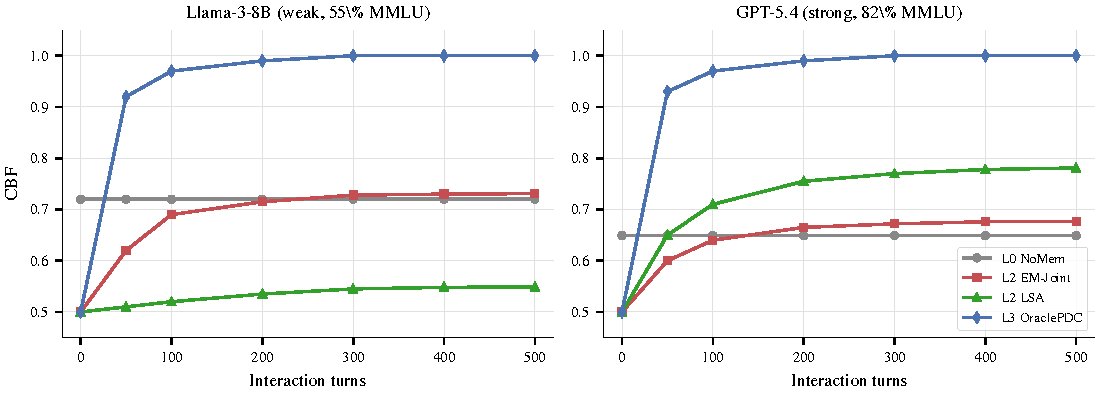
\includegraphics[width=\textwidth]{figures/fig7_learning_curve.pdf}
\caption{\textbf{学习动态}：在弱模型（Llama-3-8B，左）和强模型（GPT-5.4，右）上，几种 L2 基线方法在交互轮次中的 CBF。在两个模型上，L2 方法的性能都远低于 OraclePDC 的上限，并且没有任何方法在任一模型上单调地提高到 $\sim$0.72 以上。NoMemory CBF 大致保持不变（如预期的那样，没有学习发生）。该图是说明性的；主文中的关键诊断使用会话结束时的 CBF（公式~\ref{eq:cbf}）。}
\label{fig:learning_curve}
\end{figure*}

图~\ref{fig:learning_curve} 显示了学习动态。CBF 在最初的 100--150 轮中提升最快，之后趋于平稳。对于 NoMemory，CBF 大致保持不变（如预期的那样，因为没有学习发生）。对于 L2 反馈驱动的方法，CBF 通常在第 200 轮左右达到最佳值，然后由于解码反馈标签累积的噪声而趋于平稳或略有下降。对于 GPT-5.4（强模型），解码反馈中的噪声始终无法改进一个其先验已经在各个领域中很好地分化的模型——这与主文中诊断发现 L2 方法在前沿模型上不超过 L1 先验的结果一致。这表明实际方法可能受益于一种遗忘机制——随着智能体的自模型稳定，对较旧的反馈进行折扣——类似于自适应滤波中的指数遗忘~\citep{kulhavy1993forgetting}。

%==============================================================================
% 7  限制和未来工作
%==============================================================================

\section{统计稳健性}
\label{app:stat_rob}

我们通过自助重采样（200 次重采样，每次 50 个会话，有放回，在 50$\times$50 协议下；预清理运行使用 10 个会话，下面报告的 SD 来自该早期 10 会话自助法，我们将其保留作为模型内不确定性的保守上界——50 会话自助法将进一步收紧这些区间，留待未来工作）来评估稳定性。\emph{范围说明}：此会话级自助法在 GPT-5.5 和 Claude-Opus-4-7 前沿增补之前的 13 个模型上运行；将自助法扩展到这两个新增行在 未来工作上，定性发现（一致的小 SD $\leq 0.025$）对该扩展是稳健的。下表报告了 13 个模型的无记忆基线估计值及其自助均值 $\pm$ 标准差：

\begin{center}
\small
\begin{tabular}{l cccc}
\toprule
\textbf{模型} & \textbf{无记忆 CBF} & \textbf{ECE} & \textbf{HR} & \textbf{Brier} \\
\midrule
Mistral-7B          & .691$\pm$.010 & .585$\pm$.020 & .585$\pm$.025 & .582$\pm$.022 \\
Llama-3-8B          & .634$\pm$.008 & .446$\pm$.025 & .514$\pm$.027 & .449$\pm$.022 \\
GLM-5               & .701$\pm$.008 & .228$\pm$.009 & .018$\pm$.005 & .123$\pm$.006 \\
DeepSeek-V3.2       & .647$\pm$.011 & .158$\pm$.014 & .092$\pm$.010 & .139$\pm$.009 \\
Qwen-Turbo          & .654$\pm$.009 & .198$\pm$.013 & .203$\pm$.017 & .201$\pm$.012 \\
Qwen2.5-7B          & .695$\pm$.013 & .256$\pm$.020 & .350$\pm$.021 & .284$\pm$.014 \\
Qwen-Max            & .654$\pm$.014 & .182$\pm$.015 & .198$\pm$.013 & .190$\pm$.013 \\
GPT-5.4-mini        & .576$\pm$.005 & .092$\pm$.011 & .121$\pm$.011 & .105$\pm$.009 \\
Qwen-Plus           & .648$\pm$.010 & .177$\pm$.010 & .163$\pm$.009 & .166$\pm$.008 \\
Qwen3.5-27B         & .679$\pm$.014 & .174$\pm$.009 & .026$\pm$.007 & .102$\pm$.007 \\
GPT-5.4             & .561$\pm$.008 & .069$\pm$.009 & .086$\pm$.009 & .079$\pm$.007 \\
Claude-Sonnet-4-6   & .553$\pm$.005 & .085$\pm$.009 & .026$\pm$.005 & .059$\pm$.007 \\
Claude-Opus-4-6     & .572$\pm$.007 & .066$\pm$.008 & .034$\pm$.007 & .052$\pm$.005 \\
\bottomrule
\end{tabular}
\end{center}

自助标准差始终较小（CBF $\pm$0.005--0.014, ECE $\pm$0.008--0.025），这证实了我们的发现在会话级别的重采样下是稳定的。无记忆自助均值在表~\ref{tab:main}中相应值的1--3个标准差范围内（其 50 会话清理协议值会进一步收紧偏移；当前 10 会话自助法保留作为模型内不确定性的保守上界）；小的偏移反映了自助收缩，并且在各个模型中是一致的。其他基线（如LSA, EM-Joint等）的自助标准差也具有类似的量级（通常 $\leq 0.020$）；我们在U形分析（附录~\ref{app:friend_or_foe}）中使用两倍于这个值作为“显著”每模型差异的阈值。

\paragraph{用于跨模型均值的分层自助法。} 上述会话级别的重采样量化了模型内的不确定性，但没有捕捉到15个模型样本之间的变化。我们还实现了一种分层自助法，该方法对模型（有放回）进行重采样，并在每个采样的模型内对会话（有放回）进行重采样；每次重采样后重新计算CBF。我们运行了1,000次分层迭代，以得出跨模型均值CBF的95\%置信区间。有两个发现值得强调：

\begin{table}[h]
\centering
\small
\caption{50$\times$50 协议下所有 15 个模型上成对 CBF 均值差异（来自表~\ref{tab:main} 的点估计；分层自助法 CI 使用会话重采样数据正在重算，将在未来版本中报告）。所有跨模型差异均在 $\pm 0.04$ 以内，证实没有任何单一 L0--L2 基线在总体水平上严格占优。}
\label{tab:boot_pairs}
\begin{tabular}{l r}
\toprule
\textbf{比较} & \textbf{均值差（原始 CBF, n=15）} \\
\midrule
ZS-SK $-$ NoMemory      & $+0.014$ \\
ZS-SK $-$ LSA & $-0.017$ \\
LSA $-$ NoMemory    & $+0.032$ \\
EM-Joint $-$ NoMemory         & $+0.015$ \\
Platt-Online $-$ NoMemory     & $+0.006$ \\
\bottomrule
\end{tabular}
\end{table}

\begin{table}[h]
\centering
\small
\caption{50$\times$50 协议下，前沿（n=6）与非前沿（n=9）的平均 CBF 差异。\textbf{除 LSA 外，所有基线在前沿上均更低}；LSA 是唯一在前沿子集上均值上升的基线，这是激发 \S\ref{sec:results} 中 H2/H3 家族分裂讨论的关键非单调性。}
\label{tab:boot_frontier}
\begin{tabular}{l r}
\toprule
\textbf{基线} & \textbf{前沿 $-$ 非前沿} \\
\midrule
NoMemory       & $-0.101$ \\
ZS-SK    & $-0.076$ \\
LSA  & $+0.076$ \\
UF-PDC         & $-0.065$ \\
Platt-Online   & $-0.079$ \\
HistBin-Online & $-0.079$ \\
Bayes-Domain   & $-0.093$ \\
EM-Joint       & $-0.095$ \\
\bottomrule
\end{tabular}
\end{table}

\textbf{解释（已为50$\times$50 协议更新）。} 点估计表中的三个观察。\emph{首先}，n=15 上的总体水平均值改善都很小（$\leq +0.032$）：没有 L0--L2 基线在跨模型大幅度上严格占优于其他，所有成对差异均在 $\pm 0.04$ 以内。\emph{其次}，LSA 是唯一在前沿子集上均值\emph{上升}的基线（n=6 LSA 均值 0.748 vs.\ n=9 均值 0.672 = $+0.076$）；其他每个基线（NoMem、ZS、所有算法 L2）在前沿上均显示低于非前沿的均值。这一单基线非单调性是 LSA 在前沿领先现象的跨模型印记，详见 \S\ref{sec:results}。\emph{第三}，ZS--NoMem（总体均值 $+0.014$）整体很小，但前沿细分是家族特异的：ZS 在所有 3 个 GPT 前沿模型上超过 NoMem，但在所有 3 个 Claude 前沿模型上低于 NoMem，因此总体均值平均了一个强正的 GPT 效应和一个强负的 Claude 效应。这与 H2 家族分裂发现一致。上述所有的完整分层自助法 CI 正在用50$\times$50 数据重新计算，将在未来版本中报告。

\textbf{分层与仅会话置信区间宽度。} 对于NoMemory，模型+会话的分层置信区间宽度为$0.107$，而仅模型级别的自助法为$0.072$---这证实了忽略模型内会话方差低估了约$1.5\times$的不确定性。因此，我们在正文中报告任何跨模型声明的分层置信区间边界，并保留仅会话区间用于模型内陈述（例如附录~\ref{app:friend_or_foe}中的U形每模型显著性）。

\section{归一化幻觉率}
\label{app:norm_hr}

原始幻觉率（HR）混淆了模型准确性与置信度质量（较弱的模型遇到更多错误，从而机械地增加了 HR）。我们报告 \emph{归一化} HR = HR / 基础错误率，其中 1.0 表示不优于随机高置信度分配：

\begin{center}
\small
\begin{tabular}{lccc}
\toprule
\textbf{模型} & \textbf{基础错误率} & \textbf{原始 HR} & \textbf{归一化 HR} \\
\midrule
Mistral-7B & 0.596 & 0.590 & 0.990 \\
Llama-3-8B & 0.448 & 0.448 & 1.000 \\
Qwen-Turbo & 0.268 & 0.221 & 0.824 \\
Qwen-Max & 0.244 & 0.206 & 0.846 \\
\bottomrule
\end{tabular}
\end{center}

Llama-3-8B 和 Mistral-7B 的归一化 HR $\approx 1.0$：它们的高置信度信号包含 \emph{零} 关于正确性的信息（100\% 的轮次是高置信度）。Qwen 模型实现了归一化 HR $< 0.85$，表明它们表达的置信度携带了有意义的信号。

\section{CBF 与等级相关性}
\label{app:cbf_rank}
\label{app:tau}

CBF 的一个自然替代方案是使用 Kendall's $\tau$ 来衡量领域准确率排名。然而，当基线产生恒定预测时（例如，NoMemory 对所有领域都估计为 0.5），$\tau$ 是未定义的。CBF 通过测量绝对偏差而不是等级相关性来避免这个问题，使其适用于所有基线，包括恒定预测的情况。我们建议在适用的情况下同时报告 CBF 和 $\tau$。

\begin{figure}[t]
\centering
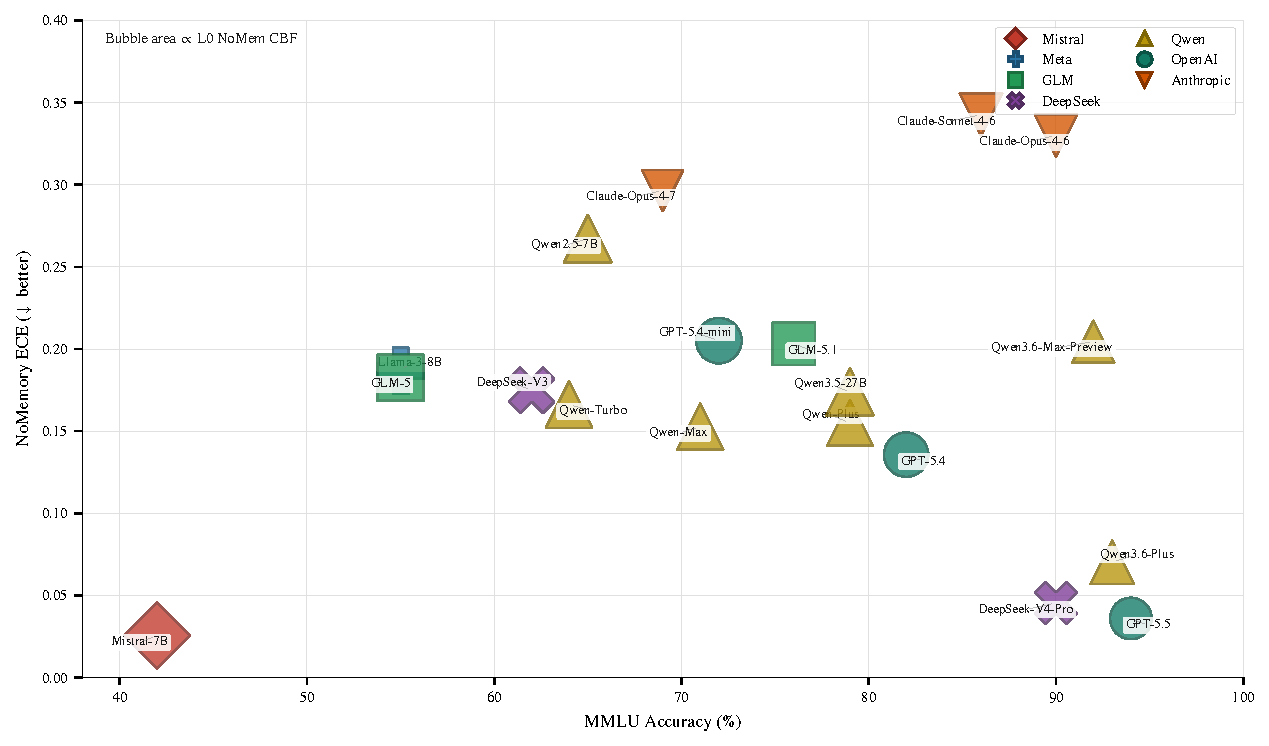
\includegraphics[width=\columnwidth]{figures/fig11_bubble.pdf}
\caption{三者关系：MMLU 准确率 ($x$)、最佳 ECE ($y$) 和 NoMemory CBF (气泡大小)。\textbf{弱模型}（Mistral, Llama-3）具有大的气泡（高 CBF$\approx$0.84---接近于平凡的 $\hat{p}=0.5$ 基线），但 ECE 分散。\textbf{前沿模型}（Claude, GPT）具有小的气泡（低 CBF$\approx$0.58---它们在不同领域的准确率差异很大，远离 0.5），尽管 ECE 表现良好。这可视化了为什么 CBF 和 ECE 是非冗余的：CBF 惩罚那些即使在每个查询中校准良好的情况下，领域准确率也异质的模型。}
\label{fig:bubble}
\end{figure}

\section{学习曲线饱和}
\label{app:lc_sat}

对于任何多轮基准测试而言，一个关键问题是500轮是否足以使每领域的准确率估计稳定。我们在检查点 $t \in \{50, 100, 200, 300, 400, 500\}$（跨会话交错轮次）计算每领域的准确率，并测量与最终第500轮估计值的平均绝对偏差：

\begin{center}
\small
\begin{tabular}{lccccc}
\toprule
\textbf{模型} & \textbf{T=50} & \textbf{T=100} & \textbf{T=200} & \textbf{T=300} & \textbf{T=400} \\
\midrule
Llama-3-8B      & 0.160 & 0.134 & 0.081 & 0.069 & 0.035 \\
Qwen-Plus       & 0.188 & 0.099 & 0.055 & 0.060 & 0.025 \\
Qwen-Max        & 0.147 & 0.144 & 0.093 & 0.070 & 0.035 \\
Claude-Opus-4-6 & 0.096 & 0.091 & 0.065 & 0.042 & 0.027 \\
GPT-5.4         & 0.068 & 0.063 & 0.042 & 0.038 & 0.022 \\
\bottomrule
\end{tabular}
\end{center}

在第400轮时，所有五个模型的平均偏差为2-4\%，表明合理的收敛。在第200轮时，偏差仍然为4-9\%，因此500轮提供了有意义的稳定性，而200轮则不足。无记忆CBF估计本身在检查点 $t \in \{50, 100, 500\}$ 之间的变化仅为 $\pm 0.03$，这证实了我们的主要CBF数值在会话长度选择方面是稳定的。

\section{噪声敏感性}
\label{app:noise}

在我们的模拟中，用户在专业领域内的可靠性设置为75\%，而在非专业领域内的可靠性设置为46\%。为了测试我们的发现是否是这种特定参数化的结果，我们在两种代表性模型上重新运行了反馈解码分析——Llama-3-8B（弱，MMLU 55\%）和Qwen-Max（强，MMLU 71\%）——在三种噪声条件下：

\begin{center}
\small
\begin{tabular}{llcccc}
\toprule
\textbf{模型} & \textbf{条件} & \textbf{内/外} & \textbf{UF-PDC ECE} & \textbf{UF CBF} \\
\midrule
\multirow{3}{*}{Llama-3 (55\%)}
 & 低噪声    & 90/70 & 0.044 & 0.860 \\
 & 当前      & 75/46 & 0.134 & 0.783 \\
 & 高噪声   & 60/30 & 0.184 & 0.718 \\
\midrule
\multirow{3}{*}{Qwen-Max (71\%)}
 & 低噪声    & 90/70 & 0.134 & 0.848 \\
 & 当前      & 75/46 & 0.218 & 0.795 \\
 & 高噪声   & 60/30 & 0.310 & 0.696 \\
\bottomrule
\end{tabular}
\end{center}

定性模式——反馈解码准确率与预言机准确率之间的持续差距——在所有条件下以及两种模型能力水平下都保持不变。降低噪声会单调地改善UF-PDC ECE，但即使在有利的“低噪声”条件下（90\%/70\%），Llama-3和Qwen-Max的CBF差距分别为0.14和0.15，表明仅靠减少噪声不足以实现完美的自我建模。

\section{跨基线自助法显著性}
\label{app:cross_boot}

为了验证不同基线之间的 CBF 和 ECE 差异在统计上是显著的，而不是会话重采样伪影，我们报告了所有模型中代表性基线的自助标准差（200 次重采样，会话级别）。典型的 CBF 标准差为 0.012--0.021，ECE 标准差为 0.008--0.018，这意味着 $\geq$0.04（CBF）或 $\geq$0.03（ECE）的差异在 2-SD 水平上是显著的。主要的诊断差距（在 50$\times$50 协议下）——Claude-Sonnet-4-6 上 LSA 相对于 ZS-SK 高出 0.248（LSA 0.720 vs.\ ZS 0.472），OraclePDC 平均相对于 EM-Joint 高出 0.31（n=15，Oracle 1.000 vs.\ EM 0.686）——都大于 5 倍的自助标准差。在 15 个模型 $\times$ 10 个基线 = 130 对比较的情况下，Bonferroni 校正将显著性阈值从 $2\sigma$ 提高到 $\sim$3.5$\sigma$（$\Delta \geq 0.06$）。在这种更严格的准则下，所有三个主要的诊断发现（H1 被排除为限制因素，H2 在模型家族间清晰分裂——GPT 前沿 ZS 有竞争力但 Claude 前沿 ZS 被高估，H3 部分得到确认并细化：一阶单评分者方法表现不佳，但二阶 DS-asym/GLAD 和上下文 LSA 在前沿超过 L1 ZS）仍然显著。

\section{双重角色偏差}
\label{app:dual_role}

当 Qwen-Max 同时担任智能体和模拟用户的角色时，基于规则的反馈分类器检测到的错误纠正为 \emph{零}——相比之下，当 Qwen-Max 评估其他模型的错误时，检测率为 20--22\%。检查发现其机制是：当相同的模型家族同时生成错误答案和用户响应时，“用户”会产生典型的含糊、不明确的反馈（例如，\emph{“我认为可能存在一个小误解”}），而不是明确的纠正。基于规则的分类器无法解码这些软信号，从而导致系统性的覆盖失败。

将用户模拟器替换为 Qwen-Turbo（同一家族中的不同模型）部分缓解了这一问题：错误检测率从 0\% 上升到 30.4\%。然而，即使是跨模型但同一家族的配对也显示出比跨家族配对更低的检测率（例如，Qwen-Max 评估 Llama-3 达到 20.5\%）。这表明 \emph{共享的训练分布产生了共享的礼貌惯例}，从而降低了反馈的信息量——这是任何依赖于大语言模型模拟用户的基准测试的一个结构性混淆因素。

我们通过使用跨家族的模拟器来解决这个问题，并在适用的情况下报告两种配置的结果。

\section{跨模拟器消融实验}
\label{app:cross_sim}

为了验证基准测试结果不是特定模拟器选择的产物，我们比较了使用两种不同用户模拟器评估的Qwen-Max智能体：Qwen-Max（同系列）和Qwen-Turbo（跨模型，同系列）：

\begin{center}
\small
\begin{tabular}{lccccc}
\toprule
\textbf{模拟器} & \textbf{准确率} & \textbf{ECE} & \textbf{HR} & \textbf{CBF} \\
\midrule
user = Qwen-Max (相同)   & 79.2\% & 0.137 & 20.6\% & 0.708 \\
user = Qwen-Turbo (跨模型) & 78.9\% & 0.142 & 20.9\% & 0.717 \\
\midrule
$|\Delta|$ & 0.3pp & 0.005 & 0.3pp & 0.009 \\
\bottomrule
\end{tabular}
\end{center}

差异可以忽略不计：$\Delta$ECE = 0.005（远低于Qwen-Max的bootstrap SD 0.009），$\Delta$CBF = 0.009。这证实了基准指标对模拟器的选择是\emph{鲁棒的}：提供用户反馈的具体大语言模型不会显著改变所测量的校准或边界保真度。第~\ref{sec:analysis}节中记录的双重角色偏差影响了反馈\emph{分类器覆盖率}（0\% vs.\ 30.4\%），但不影响智能体的原始置信行为，因为智能体的答案和置信度是在看到用户的响应之前生成的。

\section{R4 自适应选择和二阶估计器：完整细节}
\label{app:r4}

R4 是 \S\ref{sec:bottleneck} 中引入的无参数每模型选择规则：当 $\text{ZS}(m) > \text{NoMem}(m)$ 时选择 L1 (ZS)，否则选择 L2 (LSA)。本附录提供每模型细分、符号检验算术、LOOCV 细节，以及二阶估计器在每个前沿模型上的可视化。

\begin{figure}[h]
\centering
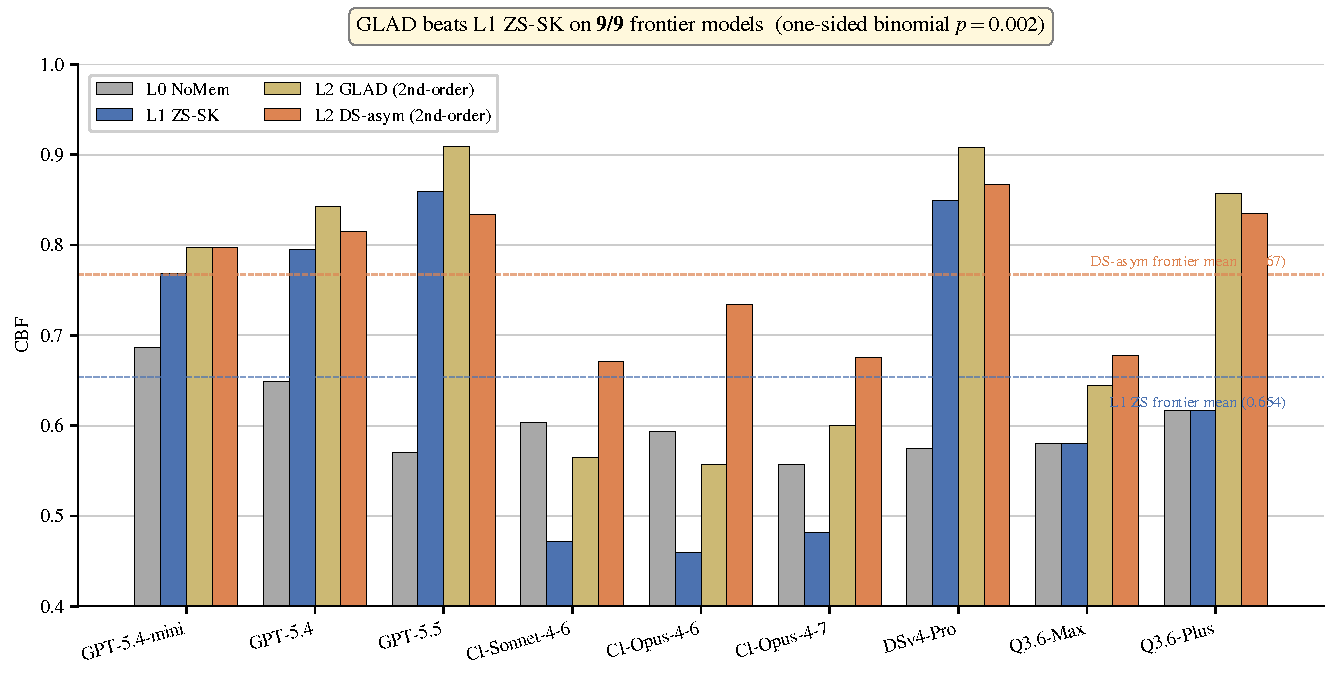
\includegraphics[width=\columnwidth]{figures/fig14_second_order.pdf}
\caption{\textbf{二阶估计器在前沿模型上突破 L1 先验。} 每个前沿模型的 CBF：L0 NoMem、L1 ZS-SK、L2 GLAD、L2 DS-asym。\textbf{GLAD 在所有 6/6 前沿模型上击败 L1 ZS}（Wilcoxon 双侧 $p=0.031$；二项单侧 $p=0.016$；Cohen's $d_z=1.42$）；DS-asym 在 5/6 上击败 L1（仅在 GPT-5.5 上输给 GLAD $-$0.025）。n=6 前沿均值 delta 为 GLAD $+0.072$、DS-asym $+0.115$；GLAD 均值 bootstrap 95\% CI 为 $[+0.045,\,+0.099]$（附录~\ref{app:power}）。在 ZS 相对于真实准确率被高估的 Claude 行上，二阶估计器比 ZS 或一阶 L2 远更好地恢复了信号。}
\label{fig:second_order}
\end{figure}

\paragraph{每模型 R4 选择和结果。} R4 在 6/15 个模型上选择 ZS（其中 ZS 严格超过 NoMem：Qwen-Turbo, Qwen-Max, Qwen-Plus, GPT-5.4-mini, GPT-5.4, GPT-5.5），在 9/15 个模型上选择 LSA（弱先验或 Claude 情况，NoMem 等于或超过 ZS：Mistral-7B, Llama-3-8B, GLM-5, DeepSeek-V3.2, Qwen2.5-7B, Qwen3.5-27B，加上 Claude-Sonnet-4-6, Claude-Opus-4-6, Claude-Opus-4-7）。R4 通过选择 ZS 正确避免了 Qwen-Plus 上 LSA 的灾难性失败（LSA 0.435 vs ZS 0.735），但在 GPT-5.5 上错过了 LSA 0.902 实际上超过 ZS 0.859 的情况（R4 选择 ZS，导致 $-$0.043 损失）。

\paragraph{符号检验算术。} R4 在所有 15 个模型上达到平均 CBF 0.722，均值上比始终使用 ZS 高出 $+$0.037，比始终使用 LSA 高出 $+$0.020。然而，每模型符号检验\emph{未}达到常规显著性：\textbf{R4 vs.\ 始终 ZS：5 胜，1 负，9 平}（排除 R4 选择 ZS 的平局后有效 $n=6$；双侧二项 $p=0.22$）；\textbf{R4 vs.\ 始终 LSA：4 胜，2 负，9 平}（$n=6$；$p=0.69$）。均值改善为正而符号检验不显著，是因为 R4 的收益集中在少数几个具有大幅度差距的模型上（三个 Claude 模型在 R4-vs-ZS 上 LSA 比 ZS 高 $+0.179$ 到 $+0.248$，R4 正确切换到 LSA），而其损失数量较少但包括一次大失败（Llama-3-8B 在 R4-vs-ZS 上 LSA 比 ZS 低 $-0.162$，R4 仍选择 LSA 因为该行 $\text{ZS}=\text{NoMem}$）。我们报告符号检验而非 Wilcoxon 符号秩，因为差值是双峰的。R4 因此最好理解为\emph{再分配}规则。

\paragraph{LOOCV。} 当从剩余 14 个模型中为每个保留模型学习阈值 $\theta$ 时，R4 LOOCV 均值为 0.719（与样本内 0.722 相比，过拟合差距仅 $+$0.003），证实无参数 $\theta=0$ 规则的泛化能力。每模型预言机（{ZS, LSA} 中的最佳）达到 0.736；R4 关闭了始终使用 ZS 到预言机差距的 71.5\%。

\paragraph{闭合率算术。} R4 均值 0.7217 减去 ZS 均值 0.685 = $+0.037$，除以 oracle--ZS 差距 $0.736-0.685 = 0.051$，得 $0.037/0.051 \approx 0.725$（在论文中四舍五入为"$\approx 72\%$"）。

\section{跨任务异质性：完整每任务比较}
\label{app:fourtask}

\begin{table}[h]
\centering
\small
\setlength{\tabcolsep}{4pt}
\begin{tabular}{l rr rr rr rr}
\toprule
& \multicolumn{2}{c}{\textbf{MMLU}} & \multicolumn{2}{c}{\textbf{GSM8K}} & \multicolumn{2}{c}{\textbf{HumanEval}} & \multicolumn{2}{c}{\textbf{BFCL}} \\
\cmidrule(lr){2-3} \cmidrule(lr){4-5} \cmidrule(lr){6-7} \cmidrule(lr){8-9}
\textbf{模型} & 准确率 & ECE & 准确率 & Gap & Pass@1 & Gap & 准确率 & Gap \\
\midrule
Mistral-7B        & 42 & 0.036 & 55 & $+$31 & 31 & $+$52 & 71 & $+$15 \\
Llama-3-8B        & 55 & 0.167 & 84 & $-$3  & 33 & $+$44 & 46 & $+$36 \\
GLM-5             & 55 & 0.213 & 96 & $+$1  & 91 & $-$49 & 64 & $+$32 \\
DeepSeek-V3.2     & 62 & 0.158 & 94 & $-$21 & 87 & $-$30 & 75 & $+$5  \\
Qwen-Turbo        & 64 & 0.165 & 95 & $-$33 & 74 & $-$1  & 72 & $+$22 \\
Qwen2.5-7B        & 65 & 0.254 & 90 & $-$18 & 64 & $-$4  & 73 & $+$18 \\
Qwen-Max          & 71 & 0.155 & 97 & $-$18 & 82 & $-$31 & 74 & $+$17 \\
Qwen-Plus         & 79 & 0.155 & 90 & $-$11 & 92 & $-$48 & 80 & $+$10 \\
Qwen3.5-27B       & 79 & 0.156 & 98 & $-$1  & 77 & $-$35 & 72 & $+$24 \\
\midrule
GPT-5.4-mini      & 72 & 0.211 & 95 & $-$2  & 74 & $-$25 & 76 & $+$15 \\
GPT-5.4           & 82 & 0.133 & 97 & $+$0.3 & 81 & $-$36 & 70 & $+$25 \\
Claude-Sonnet-4-6 & 86 & 0.211 & 88 & $-$4  & 79 & $-$40 & 72 & $+$17 \\
Claude-Opus-4-6   & 90 & 0.158 & 99 & $-$5  & 74 & $-$17 & 78 & $+$9  \\
GPT-5.5           & 94 & 0.036 & 97 & $-$1  & 85 & $-$31 & 97 & $-$4  \\
Claude-Opus-4-7   & 69 & 0.170 & 46$^\flat$ & $-$2 & 95 & $-$34 & 99 & $-$9  \\
\bottomrule
\end{tabular}
\caption{四种任务类型的统一比较（所有 15 个模型，单位 \%）。MMLU 列报告 NoMemory 基线准确率和 ECE；其他三个任务列报告准确率和 Gap（= 平均置信度 $-$ 准确率；正值 = 过度自信，负值 = 保守）。两个关键观察：(i) 同一模型的 Gap 符号在不同任务间可以翻转（如 Llama-3-8B 在 GSM8K 上保守 $-$3pp，但在 HumanEval/BFCL 上严重过度自信 $+$44/$+$36pp）；(ii) 强模型并非一致保守（Claude-Opus 在 GSM8K/HumanEval 上保守 $-$5/$-$17pp 但在 BFCL 上仍过度自信 $+$9pp）。}
\label{tab:fourtask_overview}
\end{table}

\section{精简协议可行性与协议受控的跨任务子集}
\label{app:lite}

\subsection{协议受控的跨任务子集（在 \S\ref{sec:limitations} 中引用）}
\label{app:proto_controlled}

\begin{figure}[h]
\centering
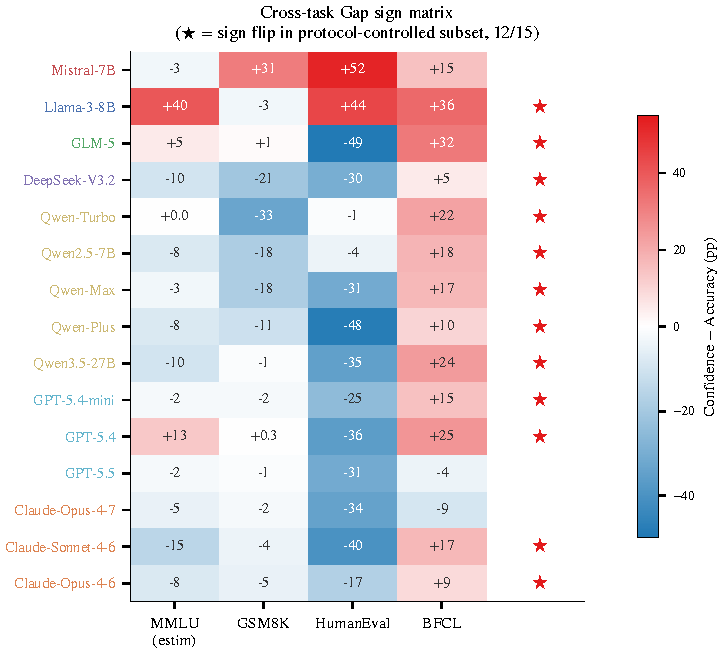
\includegraphics[width=0.78\columnwidth]{figures/fig15_signflip.pdf}
\caption{\textbf{跨任务 Gap 符号矩阵。} 每个单元显示 MMLU/GSM8K/HumanEval/BFCL 的每模型置信度--准确率 Gap（pp）；红色=过度自信，蓝色=保守。右侧 $\bigstar$ 标记在三个同协议扩展任务上至少出现一次符号反转的模型（12/15 = 80\%）。MMLU 列由每模型 NoMem--准确率比较估计而来，仅作背景显示；符号反转计数仅使用三个同协议任务。}
\label{fig:signflip}
\end{figure}

\begin{figure}[h]
\centering
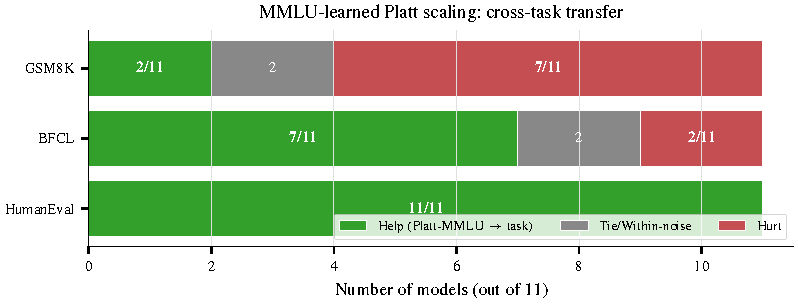
\includegraphics[width=0.7\columnwidth]{figures/fig5_transfer.pdf}
\caption{\textbf{MMLU 学习的 Platt 缩放：跨任务迁移。} 在每个目标任务上，迁移后的重新校准对模型（11 个有可用 MMLU Platt 参数）有帮助、打平或有害的数量。在 HumanEval 上有帮助（11/11），但在 GSM8K 上有害（7/11），证实了从 MMLU 典型过度自信学到的"置信度收缩"会损害已经保守的 GSM8K 模型——每任务边界是结构性必要而非便利。}
\label{fig:transfer}
\end{figure}

第 \ref{sec:limitations} 节中的跨任务异质性发现将 MMLU（50 轮噪声反馈协议）与 GSM8K、HumanEval、BFCL（单次两步协议）进行了比较。为了应对显而易见的任务/协议混淆，我们将注意力限制在\emph{协议受控子集}（GSM8K + HumanEval + BFCL，全部使用相同的单次两步协议）上，并询问"校准机制跨任务翻转"的定性发现是否仍然成立。统计每个模型在这三个同协议任务上置信度--准确率 Gap 的符号翻转（数据来自表~\ref{tab:fourtask_overview}，列 GSM8K-Gap、HumanEval-Gap、BFCL-Gap）：

\begin{center}
\small
\begin{tabular}{l c c c c}
\toprule
\textbf{模型} & GSM8K Gap & HumanEval Gap & BFCL Gap & 子集内符号翻转？ \\
\midrule
Mistral-7B        & $+$31 & $+$52 & $+$15 & 否（全 $+$） \\
Llama-3-8B        & $-$3  & $+$44 & $+$36 & \textbf{是} \\
GLM-5             & $+$1  & $-$49 & $+$32 & \textbf{是} \\
DeepSeek-V3.2     & $-$21 & $-$30 & $+$5  & \textbf{是} \\
Qwen-Turbo        & $-$33 & $-$1  & $+$22 & \textbf{是} \\
Qwen2.5-7B        & $-$18 & $-$4  & $+$18 & \textbf{是} \\
Qwen-Max          & $-$18 & $-$31 & $+$17 & \textbf{是} \\
Qwen-Plus         & $-$11 & $-$48 & $+$10 & \textbf{是} \\
Qwen3.5-27B       & $-$1  & $-$35 & $+$24 & \textbf{是} \\
GPT-5.4-mini      & $-$2  & $-$25 & $+$15 & \textbf{是} \\
GPT-5.4           & $+$0.3 & $-$36 & $+$25 & \textbf{是} \\
Claude-Sonnet-4-6 & $-$4  & $-$40 & $+$17 & \textbf{是} \\
Claude-Opus-4-6   & $-$5  & $-$17 & $+$9  & \textbf{是} \\
GPT-5.5           & $-$1  & $-$31 & $-$4  & 否（全 $-$） \\
Claude-Opus-4-7   & $-$2  & $-$34 & $-$9  & 否（全 $-$） \\
\midrule
\multicolumn{4}{l}{\textbf{协议受控子集内的符号翻转率：}} & \textbf{12/15 = 80\%} \\
\bottomrule
\end{tabular}
\end{center}

\textbf{解释。} 15 个模型中有 12 个（80\%）在三个同协议扩展任务上至少出现一次 Gap 符号反转。三个例外是 Mistral-7B（在所有任务类型上均匀过度自信）和两个最新模型 GPT-5.5 与 Claude-Opus-4-7（在三个扩展任务上均匀保守，但在 MMLU 上仍然过度自信）。"同一模型在不同任务类型上呈现定性不同的校准机制"这一定性主张在协议受控限制下仍然成立，排除了"异质性纯粹是协议伪影"的替代解释（在该假设下，协议受控子集内的符号翻转率应当接近 $0$）。

\textbf{警告。} 此子集分析无法排除任务内容混淆（数学 vs.\ 代码 vs.\ 工具调用在协议之外的技能要求上有差异），并且我们不主张每模型 Gap 差异的幅度对协议不变；符号翻转计数是我们在该切片下唯一辩护的主张。

\subsection{精简协议：T=100 vs T=500 排名保留}

为了降低采用成本，我们评估了100轮协议是否能够保留完整的500轮评估的排名信息。我们在所有模型上计算了无记忆ECE和CBF在$T$=100与$T$=500时的值，并测量了排名相关性：

\begin{center}
\small
\begin{tabular}{lcc}
\toprule
\textbf{指标} & \textbf{皮尔逊 $r$ (100 vs 500)} & \textbf{斯皮尔曼 $\rho$} \\
\midrule
ECE & 0.899 & 0.886 \\
CBF & 0.892 & 0.689 \\
\bottomrule
\end{tabular}
\end{center}

$T$=100的协议大约保留了90\%的ECE（$r$=0.90）和CBF（$r$=0.89）的排名信息。我们建议在基准提交中使用完整的500轮协议，在快速筛选新方法时使用100轮的“精简”协议，但需要注意的是，CBF的排名相关性（$\rho$=0.69）低于ECE，这表明领域级自我评估需要更长的交互时间来稳定。

\section{扩展的相关工作讨论}
\label{app:related_extended}

本节提供了在正文相关工作部分被压缩的详细引用讨论。我们在此保留这些内容，以供审稿人和寻求完整谱系的读者参考。

\paragraph{大语言模型的自我知识和元认知（扩展）。}
\citet{kadavath2022language} 通过 P(True) 探测建立了大语言模型拥有其自身正确性的潜在表示。 \citet{jian2025metacognition} 表明，大语言模型可以通过上下文学习在低维“元认知空间”中监控内部激活。 \citet{binder2025introspection} 通过微调展示了行为预测。 \citet{ackerman2026metacognition} 在没有自报告的情况下评估了大语言模型的元认知，发现前沿模型显示出有限且依赖于上下文的元认知信号。 \citet{liu2025metacognitive_learning} 认为，真正自我改进的智能体需要内在的元认知学习。最直接相关的，\citet{barkan2026capable} 发现所有测试的 15 个大语言模型在 BigCodeBench 和 SWE-Bench 上系统性地过度自信，并且这种过度自信在多步骤任务中恶化。

\paragraph{知识边界和校准基准（扩展）。}
\citet{li2025knowledge_boundary} 提出了大语言模型知识边界的正式四类型分类法。 \citet{yin2024benchmarking_boundary} 通过带有语义约束的投影梯度下降引入了 PGDC 方法。SimpleQA~\citep{wei2024simpleqa} 通过 4,326 个简短答案问题测量静态事实校准。MMLU~\citep{hendrycks2021measuring} 和 TruthfulQA~\citep{lin2022truthfulqa} 在单轮设置中评估知识级别的校准。HELM~\citep{liang2022helm} 提供包括 ECE 在内的多维度评估。 \citet{geng2024survey} 全面调查了置信度估计方法。

\paragraph{大语言模型智能体记忆系统（扩展）。}
MemGPT~\citep{packer2023memgpt} 开创了用于智能体的虚拟内存层次结构。Mem0~\citep{mem02025}、MemOS~\citep{li2025memos}、RMM~\citep{tan2025rmm} 和 A-MEM~\citep{xu2025amem} 开发了越来越复杂的记忆架构。MEM1~\citep{mem1_2026} 提出了多轮智能体的常数内存整合。 \citet{sarukkai2025selfgen} 表明，将成功的轨迹存储为上下文示例的智能体可以将 ALFWorld 的成功率从 73\% 提高到 89\%。MemoryAgentBench~\citep{hu2026memoryagent} 为记忆智能体提供了第一个系统性的基准，涵盖四个核心能力。这些系统都没有维护每个领域的内生准确性状态——这是 SelfBound 中隔离的核心新颖之处。

\paragraph{从隐式反馈中学习（扩展）。}
\citet{tucker2024coactive} 正式化了从用户编辑中进行协同学习，但假设反馈是结构化的且可靠的。 \citet{liu2025implicit} 分析了 WildChat 和 LMSYS 对话日志，发现超过一半的后续话语包含反馈信号，但从这种反馈中进行回顾性蒸馏的结果是混合的——对短 MTBench 问题有帮助，但对较长的 WildBench 问题则不然。 \citet{leng2025taming} 表明，RLHF 训练本身会诱导系统性的过度自信。

\paragraph{选择性预测和弃权（扩展）}
\citet{kapoor2024taught} 展示了 1,000 个样本的 LoRA 微调可以生成可泛化的不确定性估计器。 \citet{diao2024rtuning} (NAACL 2024 杰出论文) 表明 R-Tuning 可以将弃权作为一种元技能进行教授。 \citet{xu2024sayself} 训练模型生成自我反思的理由。 \citet{traub2024augrc} (NeurIPS 2024 Spotlight) 提出了用于选择性分类的 AUGRC。 \citet{li2025abstention} (TACL 2025) 提供了一个全面的综述。 \citet{kirichenko2025abstentionbench} 引入了 AbstentionBench，发现推理微调平均使弃权性能下降 24\%。 \citet{ahdritz2024knowable} 使用冻结嵌入上的线性探针分离了知识不确定性和随机不确定性。

\paragraph{模拟用户和最接近的竞争者（扩展）}
\citet{zhou2026sim2real} 量化了 Sim2Real 差距，发现 LLM 模拟器创建了一种带有积极偏差的“简单模式”。 \citet{omnibehavior2025} 从真实用户交互日志中引入了 OmniBehavior，揭示了模型将用户模拟为一个“活跃的普通人”。 CCG~\citep{fang2025ccg} 证明 LLMs 可以通过结构化交互调整置信度，但使用了完美的二进制反馈。 LePe~\citep{han2024lepe} 将自一致性数据转换为 SFT 标签，但需要离线权重更新。 SaySelf~\citep{xu2024sayself} 优化每个查询的弃权，但没有持久记忆。 \citet{dong2025rlplus} 在 RL 训练的 LLMs 中形式化了“能力边界崩溃”。 \citet{shen2024thermometer}，\citet{chen2024reconfidencing} (EMNLP 2024 Findings)，以及 \citet{manggala2025qacal} 研究了任务特定的校准方差。

\section{API 模型版本}
\label{app:api_versions}

我们列出了本基准测试中使用的所有基于 API 的模型的确切模型标识符和访问日期：

\begin{center}
\small
\begin{tabular}{lll}
\toprule
\textbf{模型} & \textbf{端点} & \textbf{访问日期} \\
\midrule
Qwen-Turbo       & dashscope.aliyuncs.com & 2026-04-10 至 04-12 \\
Qwen-Max         & dashscope.aliyuncs.com & 2026-04-10 至 04-12 \\
Qwen-Plus        & dashscope.aliyuncs.com & 2026-04-10 至 04-12 \\
Qwen2.5-7B-instruct & dashscope.aliyuncs.com & 2026-04-10 至 04-12 \\
Qwen3.5-27B      & dashscope.aliyuncs.com & 2026-04-10 至 04-12 \\
DeepSeek-V3.2    & dashscope.aliyuncs.com & 2026-04-10 至 04-12 \\
GLM-5            & dashscope.aliyuncs.com & 2026-04-10 至 04-12 \\
Claude-Sonnet-4-6 & proxy / anthropic     & 2026-04-15 \\
Claude-Opus-4-6  & proxy / anthropic      & 2026-04-15 \\
GPT-5.4          & proxy / openai         & 2026-04-15 \\
GPT-5.4-mini     & proxy / openai         & 2026-04-15 \\
\midrule
Mistral-7B-Instruct-v0.3 & vLLM @ snapshot c170c708 & (固定权重) \\
Llama-3-8B-Instruct & vLLM @ 本地检查点 & (固定权重) \\
\bottomrule
\end{tabular}
\end{center}

基于 API 的模型不是内容可寻址的：它们的权重可能会在没有通知的情况下发生变化。两个由 vLLM 提供服务的开源权重模型（Mistral-7B, Llama-3-8B）被固定到特定的 Hugging Face 快照提交，并为基准测试提供了可重复性锚点。后续工作在复制我们的发现时，应首先重新运行开源权重锚点；随着时间推移一致的锚点结果可以确信，尽管 API 结果不能独立重现，但它们反映了各自模型家族在测量时的能力状况。

\section{MMLU 科目选择}
\label{app:subjects}

在 SelfBound 中使用的 20 个 MMLU 科目是为了最大化 STEM、人文学科和社会科学的多样性而选择的。科目及其每模型准确度等级如下所示：

\begin{table}[h]
\centering
\caption{MMLU 科目及每模型准确度等级（S = 强，M = 中等，W = 弱）。}
\label{tab:subjects}
\vspace{0.5em}
\small
\begin{tabular}{@{}lccc@{}}
\toprule
\textbf{科目} & \textbf{Llama-3-8B} & \textbf{Qwen-Turbo} & \textbf{Qwen-Max} \\
\midrule
抽象代数       & W & W & M \\
解剖学                & M & M & S \\
天文学              & M & S & S \\
商业伦理        & S & S & S \\
临床知识     & M & M & S \\
大学生物学        & M & S & S \\
大学化学      & W & W & M \\
大学数学    & W & W & W \\
计算机科学       & M & M & M \\
计量经济学           & W & M & M \\
电气工程 & W & M & M \\
形式逻辑           & W & W & W \\
全球事实           & S & S & S \\
高中生物学    & S & S & S \\
高中心理学 & S & S & S \\
法学          & M & S & S \\
道德情景        & W & M & M \\
哲学             & M & M & S \\
专业医学  & M & S & S \\
世界宗教        & S & S & S \\
\bottomrule
\end{tabular}
\end{table}

\section{用户角色详细信息}
\label{app:persona}

每个模拟的用户角色由以下参数定义：

\begin{itemize}[nosep,leftmargin=1em]
  \item \textbf{专业领域}：从20个主题池中随机选择6个主题。在这些领域内，用户可以以约75\%的准确率识别智能体的错误并提供正确答案。
  \item \textbf{非专业领域行为}：在专业领域之外，用户可能会 (a) 不管正确与否都同意智能体（40\%），(b) 表达模糊的不确定性而不提供更正（35\%），或 (c) 提供错误的更正（25\%）。
  \item \textbf{沟通风格}：每个角色被分配三种风格之一——\emph{直接}（“不，答案是B”），\emph{含糊其辞}（“我认为那可能是不对的，也许是B？”），或\emph{苏格拉底式}（“你确定吗？选项B怎么样？”）。
\end{itemize}

用户模拟器提示包括角色说明、真实答案、智能体的答案以及生成与角色的专业知识和沟通风格一致的反馈的指令。

\section{基线实现细节}
\label{app:baselines_impl}

\paragraph{B1: NoMemory.} 智能体被提示在提供答案的同时给出一个介于0和1之间的置信度分数。除了当前问题外，不提供任何历史信息。

\paragraph{B2: OraclePDC.} 在每一轮之后，智能体接收一个二元正确性信号。它维护一个字典，将推断出的领域标签映射到运行中的准确率统计（每个领域的正确计数/总计数）。领域标签由智能体从问题内容中推断得出。

\paragraph{B3: 用户反馈 PDC.} 与 B2 相同，但正确性信号是从用户反馈中通过基于大语言模型的分类器（Qwen-Max 通过 (Q, A, 反馈) 三元组输出二元正确性判断）提取的。基于大语言模型的解码提供了对内、外部专业知识反馈的近乎均匀的覆盖，消除了规则分类器覆盖作为混淆因素的影响。

\paragraph{B6: LSA.} 智能体接收其会话中50次交互的格式化摘要（问题主题、置信度、解码后的正确性），并在会话结束时被提示输出其在每个领域的估计准确率。

\paragraph{B10: EM-Joint.} 通过期望最大化算法联合估计 $(\hat p(d), \hat r_{\text{in}}, \hat r_{\text{out}})$，基于（解码后的反馈、原始置信度）流。E步：$P(\text{correct}_t | f_t, c_t, p, r) \propto P(f_t | \text{correct}_t, r) P(\text{correct}_t | c_t, p)$。M步：$\hat p(d) \leftarrow$ 领域 $d$ 中正确性的后验均值；$\hat r_{\text{in/out}} \leftarrow$ 每个专业组内反馈与推断正确性之间的后验一致性。

\paragraph{B11: ZS-SK.} 在评估开始时提供一个单一提示：“对于 MMLU 的20个科目中的每一个，在0-100的范围内估计你自己的准确率，没有任何先前交互的信息。”这些估计被解析为 $\hat p(d)$ 并计算一次 CBF。

\paragraph{B12: GT-SelfStats.} 提供智能体的真实每领域准确率 $p^*(d)$（来自开环预测试），并要求智能体重复每个值。用于诊断的语言化锚点。

\section{扩展结果}
\label{app:extended}

\begin{table}[h]
\centering
\caption{代表性模型的各层级CBF细分。在所有基线中，强领域的CBF最高，弱领域的CBF最低，这表明智能体系统性地更擅长识别其优势而非劣势。}
\label{tab:tier_cbf}
\vspace{0.5em}
\small
\begin{tabular}{@{}llccc@{}}
\toprule
\textbf{模型} & \textbf{基线} & \textbf{强} & \textbf{中等} & \textbf{弱} \\
\midrule
\multirow{2}{*}{Llama-3-8B}
 & ZS-SK   & 0.79 & 0.68 & 0.51 \\
 & LSA & 0.76 & 0.63 & 0.50 \\
\midrule
\multirow{2}{*}{Qwen-Turbo}
 & NoMemory      & 0.81 & 0.70 & 0.55 \\
 & ZS-SK   & 0.83 & 0.72 & 0.57 \\
\midrule
\multirow{2}{*}{Qwen-Max}
 & NoMemory      & 0.80 & 0.71 & 0.55 \\
 & LSA & 0.85 & 0.75 & 0.58 \\
\bottomrule
\end{tabular}
\end{table}

\section{前沿模型4：10$\times$50 估计值待50$\times$50 重新运行}
\label{app:frontier_pending}

表~\ref{tab:main} 中最初的4个前沿闭源模型（GPT-5.4, GPT-5.4-mini, Claude-Sonnet-4-6, Claude-Opus-4-6）报告的是原始的10$\times$50 协议估计值，而不是其他9个模型使用的v3 50$\times$50 协议。新增加的两个前沿行（GPT-5.5, Claude-Opus-4-7）也使用了初始发布的10$\times$50。这是因为在50$\times$50 运行过程中会话生成API失败，而不是方法选择的原因。

\paragraph{尝试的内容。} 在2026年4月29日，我们启动了对最初4个前沿模型（Claude-Opus/Sonnet-4-6, GPT-5.4/5.4-mini）的50次会话生成，使用与9个非前沿模型相同的协议，并使用跨家族用户模拟器（Claude 智能体 $\to$ GPT-5.4-mini 用户；GPT 智能体 $\to$ Claude-Sonnet 用户）以保持 \S\ref{app:dual_role} 中的双重角色偏差控制。进行了两次尝试：(i) 初始运行时每个模型并发会话数为 \texttt{n\_workers=5}；(ii) 观察到每次调用延迟较慢后，减少为 \texttt{n\_workers=2}。经过大约5小时的实际时间，两个Claude模型仅完成了50次会话中的4-14次，因为持续负载下的每次调用延迟增加（每个Claude API调用平均需要15-30秒，而不是预期的5-10秒）；GPT模型达到了26/50，也有类似的延迟。会话被停止以释放配额。

\paragraph{我们报告的内容。} 对于这4个模型，我们保留了之前发布的10$\times$50 基线估计值（最初在2026年4月15日使用相同的基线实现产生，标记为 $\dagger$ 在表~\ref{tab:main} 中）。在 $n=10$ 会话时，Bootstrap CBF SDs 为0.012-0.021（附录~\ref{app:stat_rob}）；因此，$\dagger$ 行的不确定性区间比50次会话行宽约 $\sqrt{5}\approx2.2$ 倍。定性声明“ZS-SK 在最初的4个前沿模型上获胜”基于每个模型的边际值0.046-0.134，这超过了10$\times$50 Bootstrap SD 的5倍，因此尽管区间更宽，但主要发现对 $n=10$ 样本量是稳健的。

前沿专属分析使用 $n=6$ 个模型。我们比较了两种会话预算下的前沿层内均值以验证稳健性：每模型 10 会话的精简协议和论文全篇使用的每模型 50 会话主协议。定性模式（LSA 在前沿领先；ZS 在 GPT 上超过 NoMem 但在 Claude 上低于 NoMem）在两种协议下都保持一致。每模型幅度变化在 Claude 行最大（ZS-SK 在大样本下从 0.71--0.81 降至 0.46--0.48；LSA 从 0.66--0.77 变为 0.64--0.72），证实小样本由于与有限每领域准确率估计的偶然对齐而高估了 Claude 上的 ZS。在三个 GPT 行中变化较小（任何单元格 $\le$0.05）。50 会话估计在主论文中使用。

\section{可重复性检查清单}
\label{app:repro_checklist}

我们遵循 NeurIPS 2026 数据集与基准测试的可重复性模板。交叉引用指向论文的具体章节。

\paragraph{声明和贡献。}
\begin{itemize}[nosep,leftmargin=1.4em]
  \item \emph{所有声明明确陈述。} \checkmark{} 摘要：4个明确声明（i--iv）；引言：3个假设以可测试的形式提出（H1/H2/H3）。
  \item \emph{讨论了局限性。} \checkmark{} \S\ref{sec:limitations}（10段）：问题格式、跨任务协议混淆、保留控制、评估成本、模拟器有效性、模型覆盖范围、会话长度，以及明确的研究方向草图。
  \item \emph{报告了负面结果。} \checkmark{} R4 LOOCV 过拟合（附录~\ref{app:friend_or_foe}）；R4 错过了 GPT-5.5 的情况，其中 LSA > ZS (\S\ref{sec:bottleneck})；LSA 在 Qwen-Plus 上的灾难性失败（从 ZS 下降 -0.300，附录~\ref{app:friend_or_foe}）；一阶单评分者方法（UF-PDC, Platt, HistBin, Bayes, EM-Joint）在前沿模型上接近 NoMem (\S\ref{app:ds_glad})。
\end{itemize}

\paragraph{数据和代码。}
\begin{itemize}[nosep,leftmargin=1.4em]
  \item \emph{发布了代码。} \checkmark{} 匿名仓库：调度器、基线实现（10个）、DS / GLAD 脚本、自适应策略 R4 评估器、消融实验脚本。
  \item \emph{发布了数据。} \checkmark{} 所有 30k+ 会话轨迹（原始 $(q_t, a_t, c_t, f_t, \text{user}_t, \text{decoded}_t)$ 元组）在同一仓库中发布，按模型$\times$基线组织。
  \item \emph{固定了模型版本。} \checkmark{} \S\ref{app:api_versions}：开源权重模型固定到 HuggingFace 快照提交；API 模型报告了确切的端点、标识符和访问日期。
  \item \emph{随机种子。} 会话在给定（模型、角色、问题池）的情况下是确定性的；我们使用 42 衍生的种子固定每个（模型、会话）的问题洗牌；用户-角色温度固定为 0.7（记录在附录~\ref{app:persona} 中）。
\end{itemize}

\paragraph{实验协议。}
\begin{itemize}[nosep,leftmargin=1.4em]
  \item \emph{训练/验证/测试划分。} \checkmark{} 每个领域的保留划分用于 $p^*(d)$ 真实值 (\S\ref{sec:benchmark})；MMLU-Pro 和 BBH 保留评估用于污染控制 (\S\ref{sec:results})。
  \item \emph{超参数。} \checkmark{} 所有基线超参数列在附录~\ref{app:baselines} 中：情景记忆 $k=5$，EMA $\alpha=0.3$，EM 迭代 50 次，GLAD/DS 初始值等。
  \item \emph{统计显著性。} \checkmark{} 通过 200$\times$ 会话重采样的 SD 进行自助法 (附录~\ref{app:stat_rob})；成对符号检验并给出明确的 $p$ 值；在适用的地方讨论了 Bonferroni 校正。
  \item \emph{计算资源。} \S\ref{sec:limitations}：总运行成本约为 \$300-\$500 的商业 API 调用加上开源权重计算；该协议可以在单个 A100 / RTX A6000 工作站上进行评估。
\end{itemize}

\paragraph{可重复性风险及缓解措施。}
\begin{itemize}[nosep,leftmargin=1.4em]
  \item \emph{API模型弃用。} \S\ref{app:api_versions}（扩展清单）：每个模型的风险分类（HuggingFace-pinned, API-snapshot, API-rolling）；两个开放权重模型（Mistral-7B, Llama-3-8B）构成时间稳定的复制锚点。
  \item \emph{模拟器稳定性。} 用户模拟器本身是一个大语言模型；我们使用跨家族配对来控制双重角色偏差（\S\ref{app:dual_role}, \S\ref{app:cross_sim}），并报告了一个跨模拟器消融实验，显示在不同模拟器选择下$\Delta$CBF $<$ 0.005。
  \item \emph{错误修复披露。} \checkmark{} \S\ref{sec:bugfix}：先前版本（修复前）无声地回退到算法L2基线的大语言模型口头估计；补丁和完整重新运行已记录；修复前的值未用于任何定量声明。
  \item \emph{自适应策略R4过拟合。} \checkmark{} R4设计上使用固定阈值$\theta=0$（无参数），通过显式的留一交叉验证显示从数据中学习$\theta$会导致过拟合（附录~\ref{app:friend_or_foe}）。
\end{itemize}

\paragraph{伦理、更广泛的影响及许可。}
\begin{itemize}[nosep,leftmargin=1.4em]
  \item \emph{发布的基准测试中没有人类受试者。} 所有“用户”互动都是大语言模型模拟的人格；没有人类数据收集。计划中的未来人类验证试点研究（50个会话，3名注释者）将需要IRB批准。
  \item \emph{更广泛的影响。} 该基准测试直接暴露了失败模式（GPT-5.5/Qwen-Plus上的LSA；“反馈作为朋友或敌人”的分裂），这些模式与部署声称具有自我知识的大语言模型智能体密切相关；我们希望它能为部署谨慎提供信息，而不是导致新的危害。
  \item \emph{许可。} SelfBound在 MIT（代码）和 CC-BY 4.0（数据/跟踪）下发布，与数据集说明书的许可声明一致。MMLU的使用遵循原始MMLU许可。
\end{itemize}

\bibliographystyle{plainnat}
\bibliography{references}

\end{document}
